\documentclass[/Users/ikedahajime/GitHub/reserch/master_report/thesis]{subfiles}
% このファイル内だけのコマンド
\begin{document}
\chapter{結果}
% \section{はじめに}
%TODO:全体として、軸に対する言及をつける
本章では計算結果および解析結果を述べる。
\secref{sec:result_abp}ではABPを、\secref{sec:result_cabp}ではCABPを
それぞれ壁の中に閉じ込めた時の結果について述べる。
\section{円に拘束されたABP}\label{sec:result_abp}
本節では、ABPを円形領域に閉じ込めた時の結果を示す。
\subsection{系全体のダイナミクス}\label{subsec:result_nabp_holedinamics}
\subsubsection{低密度系}
本節では低密度系である$\varphi=0.5$における系の流れについて論ずる。
\figref{fig:nabp_coor_lodense_mlo_taudep}は粒子のスナップショットである。パラメータは
$M=0.1$の慣性の影響が小さな系を用い、$Pe$による違いを示した。
%TODOずをみて論じる:図に使ったパラメータの説明
\begin{figure}
    \centering
    \begin{tabular}{c}
        \begin{minipage}{0.3\hsize}
            \text{(a)}
            \includegraphics[width=\textwidth]{img/nabp/recap_mss_ani/arrR10_lo0.5_tau0.1_ms0.1.pdf}
        \end{minipage}\begin{minipage}{0.3\hsize}
            \text{(b)}
            \includegraphics[width=\textwidth]{img/nabp/recap_mss_ani/arrR10_lo0.5_tau10.0_ms0.1.pdf}
        \end{minipage}
        \begin{minipage}{0.3\hsize}
            \text{(c)}
            \includegraphics[width=\textwidth]{img/nabp/recap_mss_ani/arrR10_lo0.5_tau100.0_ms0.1.pdf}
        \end{minipage}

    \end{tabular}
    \caption[coor_lo]
    {
        $\varphi=0.5、R=10$における粒子配置。各図において、粒子の色は各粒子の角運動量を表す。
        パラメータは$M=0.1$の慣性の影響が小さい系を用い、(a) $Pe=0.1$ (b) $Pe=10$ (c) $Pe=100$ である。
    }
    \label{fig:nabp_coor_lodense_mlo_taudep}
\end{figure}

まず$M=0.1$の慣性による影響が小さい領域を見る。\figref{fig:nabp_coor_lodense_mlo_taudep} を見ると、
$Pe$が小さな領域では粒子は空間に一様に分布しており、$Pe$が大きくなるに従って粒子は壁付近に凝集していることが
わかる。
これは ABP において観測されている障害物への集積\cite{yangAggregationSegregationConfined2014}
と同様の現象である。この現象は MIPS\cite{filyAthermalPhaseSeparation2012}
と同じ原理で発生していると考えられる。これは壁に向かって進もうとする ABP を考えるとわかる。
この ABP が1粒子の場合、粒子は壁に衝突したことによってその進行方向を変えないため、
典型的に時間$\tau_p$の間壁付近に留まり続け、その後進行方向を変えて壁付近から離れる。
一方多粒子系においては、壁付近に止まっている間に他の粒子が重なり、壁付近からの脱出を妨害するため、
結果として粒子は壁付近に層をなして積み重なる。%TODO:つなぎ

この低慣性系におけるオーダーパラメータ$\psi、V$は\figref{fig:nabp_lodense_lom_taudep_timedep}のようになった。
\begin{figure}
    \centering
    \begin{tabular}{c}
        \begin{minipage}{0.3\hsize}
            \text{(a)}
            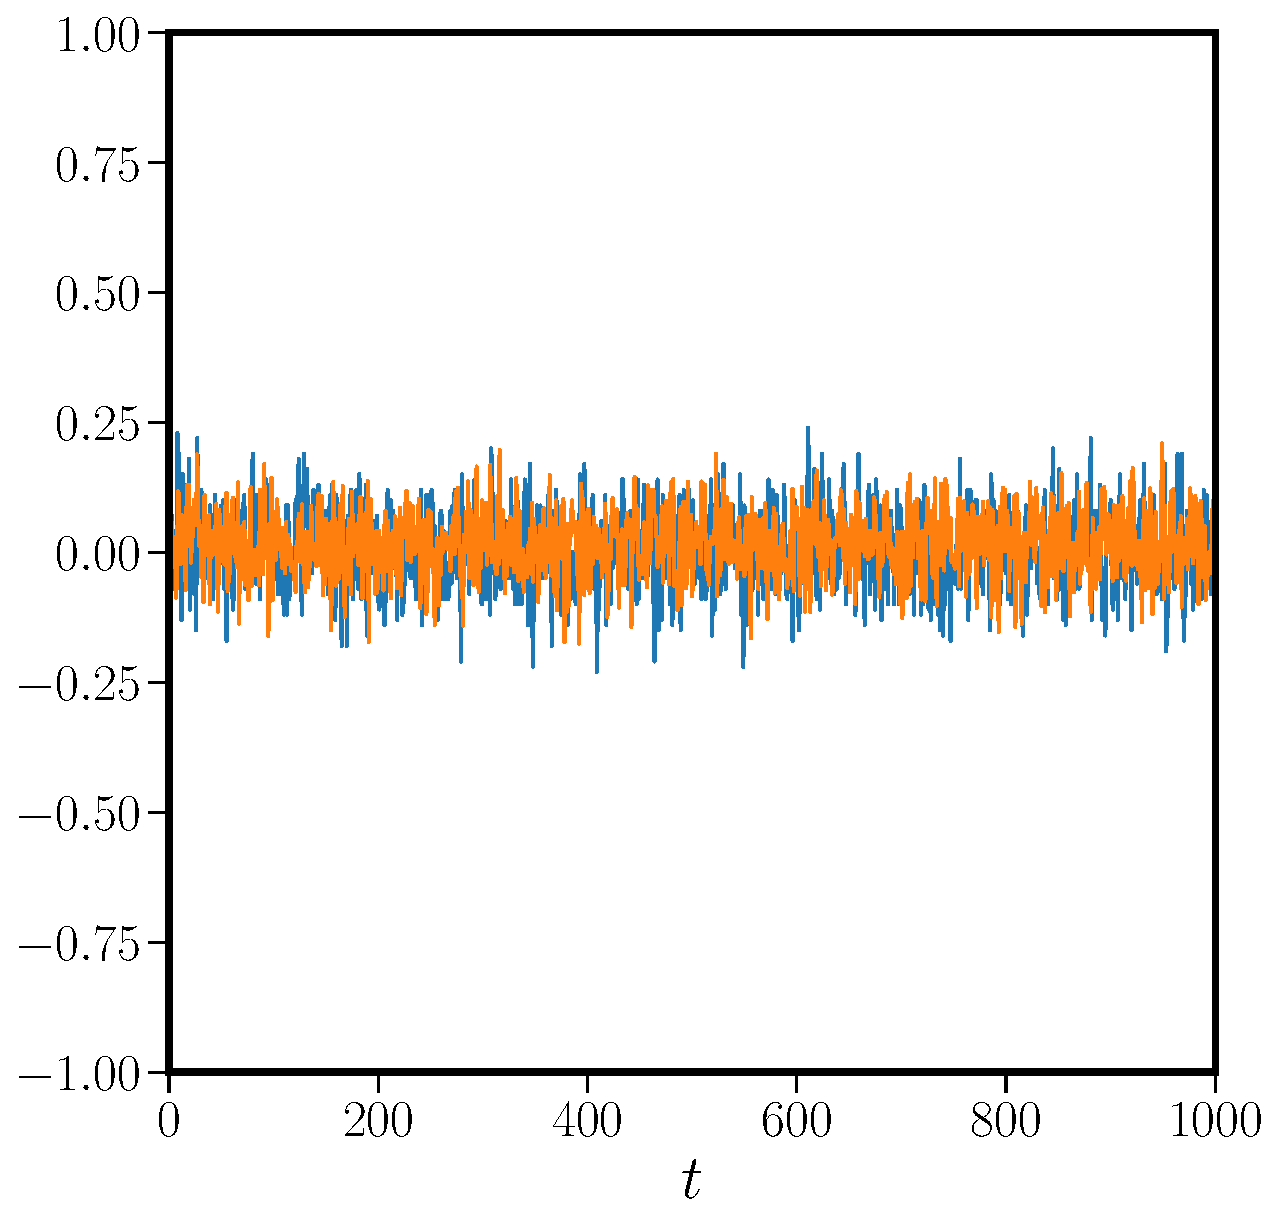
\includegraphics[width=\textwidth]{img/nabp/recap_mss/orderparameter_0.5_0.1_tau0.1.pdf}
        \end{minipage}
        \begin{minipage}{0.3\hsize}
            \text{(b)}
            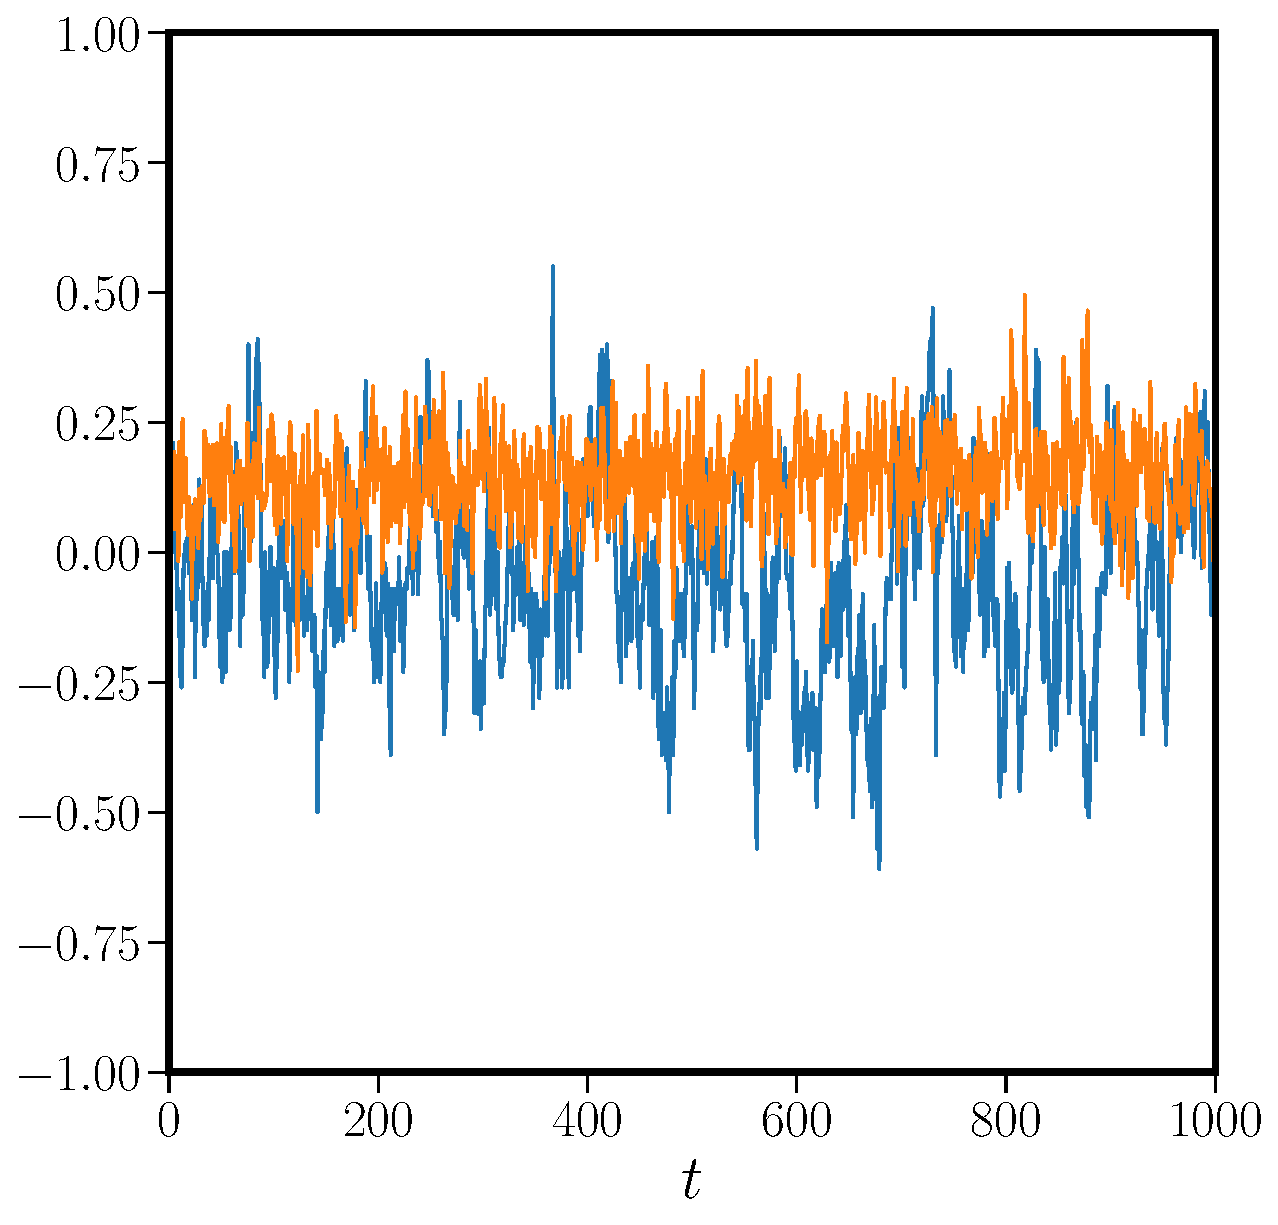
\includegraphics[width=\textwidth]{img/nabp/recap_mss/orderparameter_0.5_0.1_tau10.pdf}
        \end{minipage}
        \begin{minipage}{0.3\hsize}
            \text{(c)}
            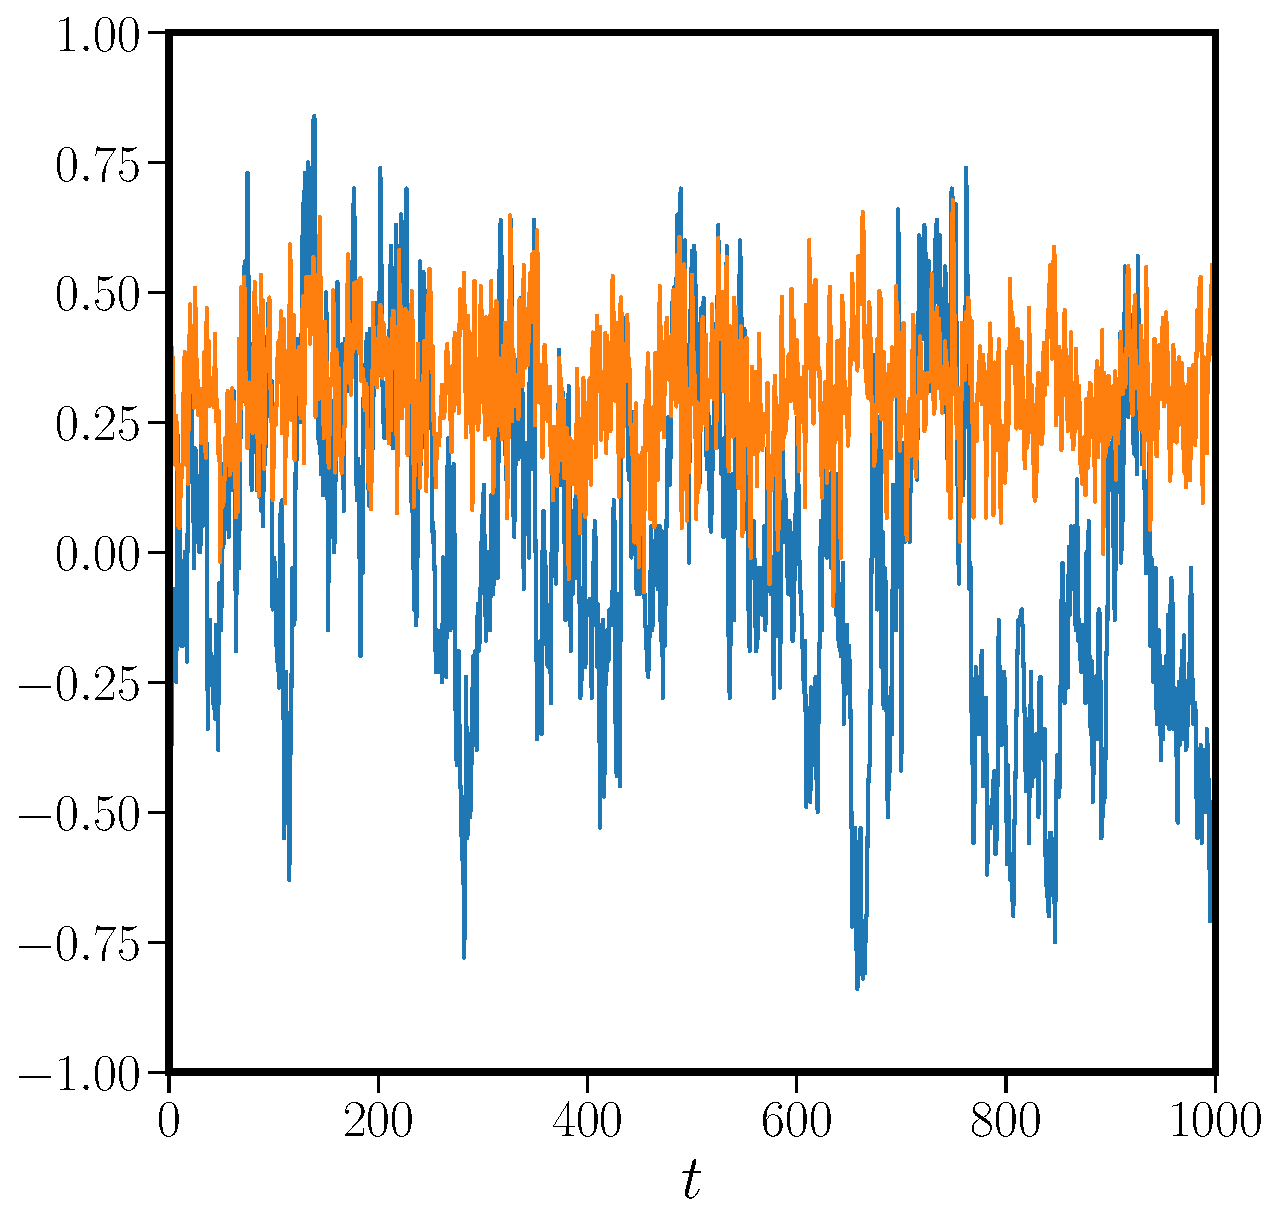
\includegraphics[width=\textwidth]{img/nabp/recap_mss/orderparameter_0.5_0.1_tau100.pdf}
        \end{minipage}
    \end{tabular}
    \caption[timedep_lolom]
    {
        オーダーパラメータの時間依存性。オレンジ色の線は$\psi(t)$を、青色の線は$V(t)$を表す。
        パラメータは$\varphi=0.5、R=10、M=0.1$とし、(a) $Pe=0.1$ 、(b) $Pe=10$、(c) $Pe=100$とした。
    }
    \label{fig:nabp_lodense_lom_taudep_timedep}
\end{figure}
この図から、$Pe$が小さい$Pe=0.1$の系では$\psi、V$が共に0付近であり、これは系全体で無秩序な運動をしていることを表す。
$Pe$が大きな$Pe=10、Pe=100$の領域においては$V$の絶対値が1に近く系全体で流れが生じているように見える。
しかし、これらの領域においては MIPS が発生している。
そのため動き回る粒子が少ない。ここで、$\psi$の定義\equref{eq:def_psi}から、
この変数は速度の総和に対する、角度方向の速度の絶対値の総和の比を用いて表されるオーダーパラメータである。
つまり、少数の粒子による運動の効果が、その他の粒子による運動の効果に比べて大きい時、
この少数の粒子による影響を強く受ける。そのため$\psi$はこの領域の解析に適さない。
また、$|V|$の値も大きくなるが、これは壁に集まった粒子が一斉に動くことで起こっている現象で、これは系全体における渦ということはできない。
つまり、この系では壁付近に粒子が密集する MIPS が見られたが、この MIPS は系の流れを解析する場合にその流れを隠す働きがある。
そのため、MIPS の影響を避けるために慣性$M$の効果を大きくした系、及び高密度系について解析を行なった。%TODO:これはMIPSだからダメ


\begin{figure}
    \centering
    \begin{tabular}{c}
        \begin{minipage}{0.3\hsize}
            \text{(a)}
            \includegraphics[width=\textwidth]{img/nabp/recap_mss_ani/arrR10_lo0.5_tau0.1_ms80.0.pdf}
        \end{minipage}\begin{minipage}{0.3\hsize}
            \text{(b)}
            \includegraphics[width=\textwidth]{img/nabp/recap_mss_ani/arrR10_lo0.5_tau10.0_ms80.0.pdf}
        \end{minipage}
        \begin{minipage}{0.3\hsize}
            \text{(c)}
            \includegraphics[width=\textwidth]{img/nabp/recap_mss_ani/arrR10_lo0.5_tau100.0_ms80.0.pdf}
        \end{minipage}

    \end{tabular}
    \caption[coor_lo]
    {
        $\varphi=0.5、R=10$における粒子配置。各図において、粒子の色は各粒子の角運動量を表す。
        パラメータは$M=80$を用い、(a) $Pe=0.1$ (b) $Pe=10$ (c) $Pe=100$ である。
    }
    \label{fig:nabp_coor_lodense_mhigh_taudep}
\end{figure}
\figref{fig:nabp_coor_lodense_mhigh_taudep}は慣性が大きい$M=80$における粒子配置である。
\figref{fig:nabp_coor_lodense_mlo_taudep}とこの図を比べると、
慣性が小さい系において MIPS が発生していた$Pe$においても粒子分布は一様であり、MIPS が見られない。
これはバルク系においても見られる現象\cite{kurodaAnomalousFluctuationsHomogeneous2023}である。%TODOiabpの最初を確認,原理について解説?
これはこのパラメータにおけるオーダーパラメータ\figref{fig:nabp_lodense_him_taudep_timedep}を見ることでも理解することができる。
まず$\psi$の値に注目すると、いずれの$Pe$においてもその値は常に0に近い。
このことから、すべての粒子が無秩序な方向に運動していることが分かる。%TODO何か二言
つまり、慣性が大きく密度が低い系においては円の中に流れは発生しないことが分かる。
\begin{figure}
    \centering
    \begin{tabular}{c}
        \begin{minipage}{0.3\hsize}
            \text{(a)}
            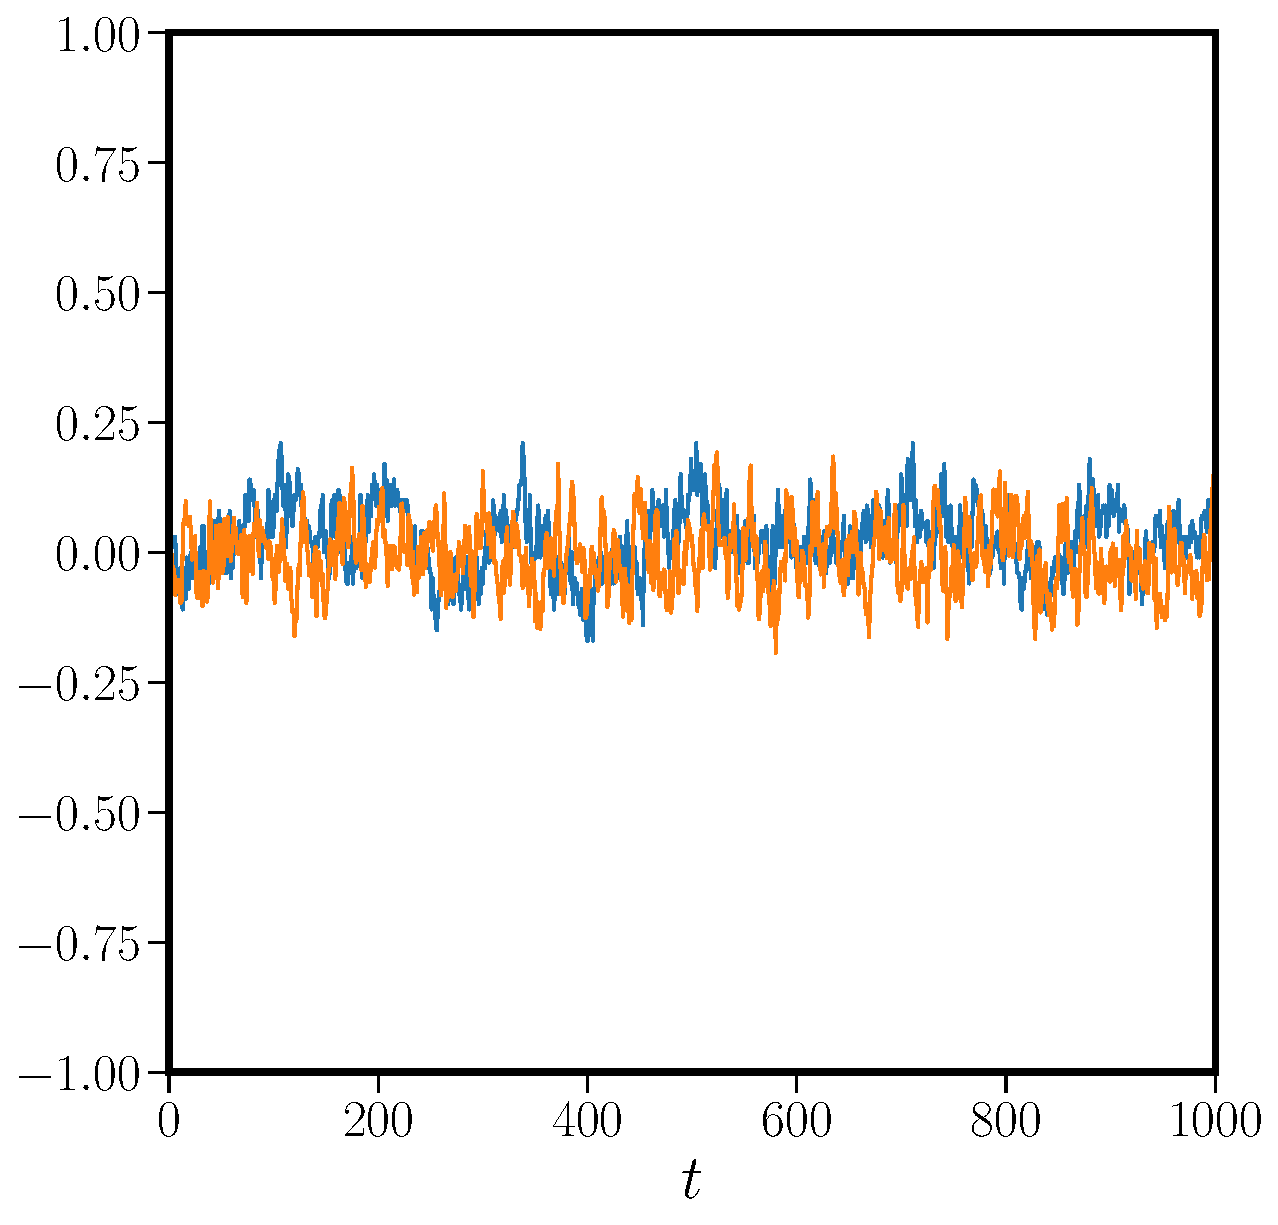
\includegraphics[width=\textwidth]{img/nabp/recap_mss/orderparameter_0.5_80_tau0.1.pdf}
        \end{minipage}
        \begin{minipage}{0.3\hsize}
            \text{(b)}
            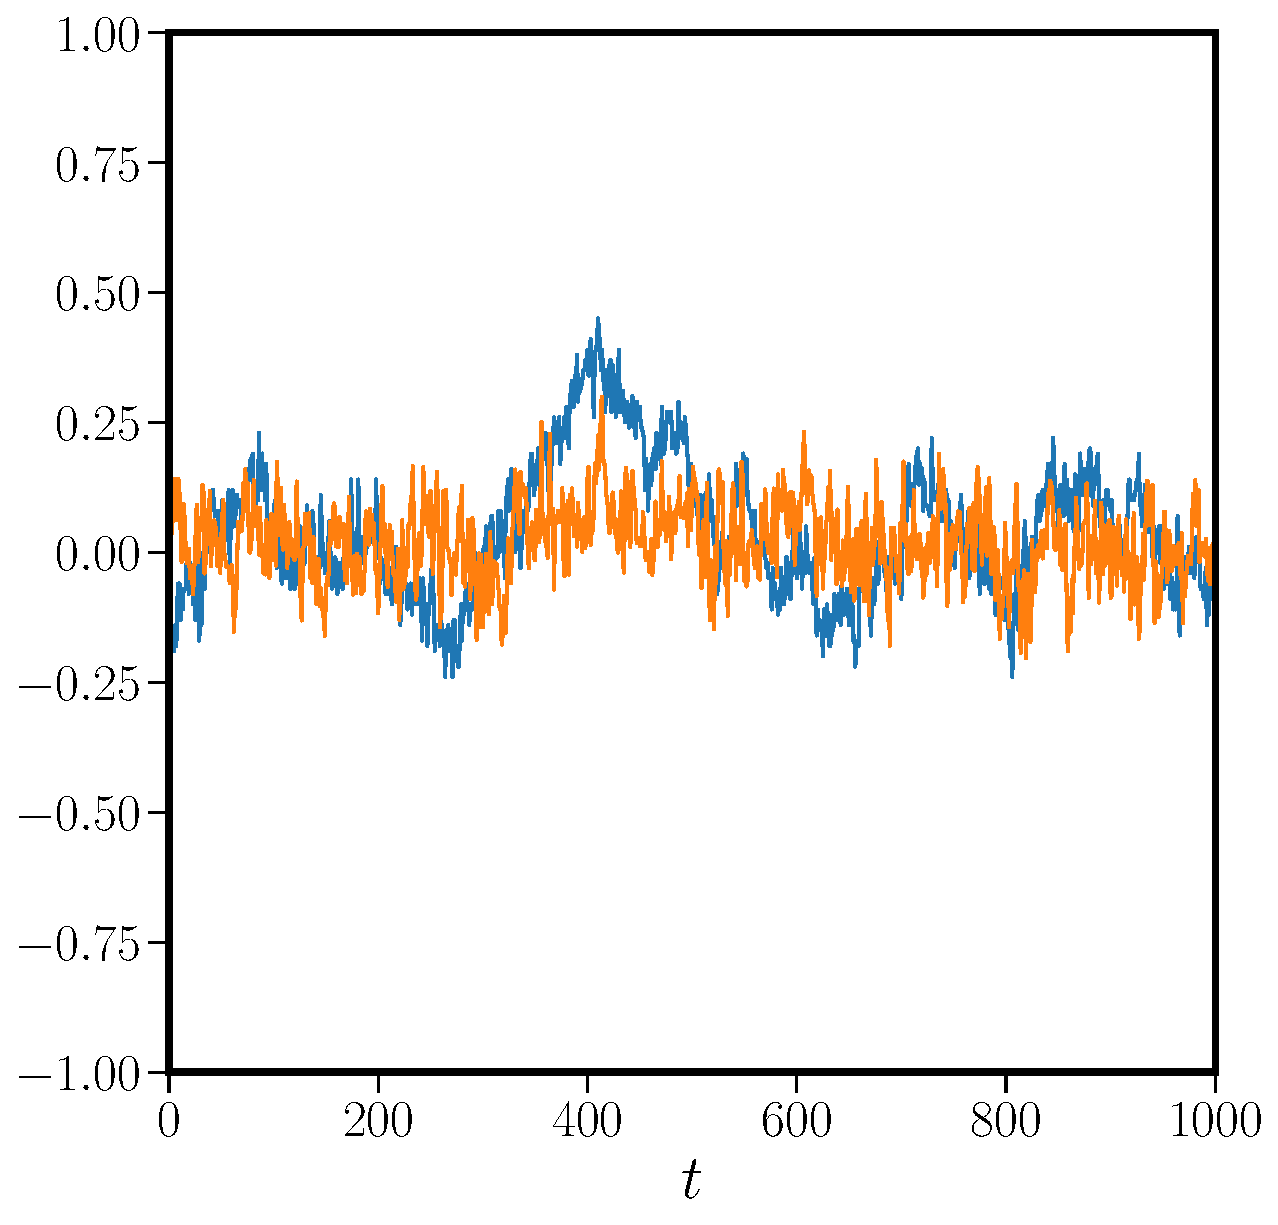
\includegraphics[width=\textwidth]{img/nabp/recap_mss/orderparameter_0.5_80_tau10.pdf}
        \end{minipage}
        \begin{minipage}{0.3\hsize}
            \text{(c)}
            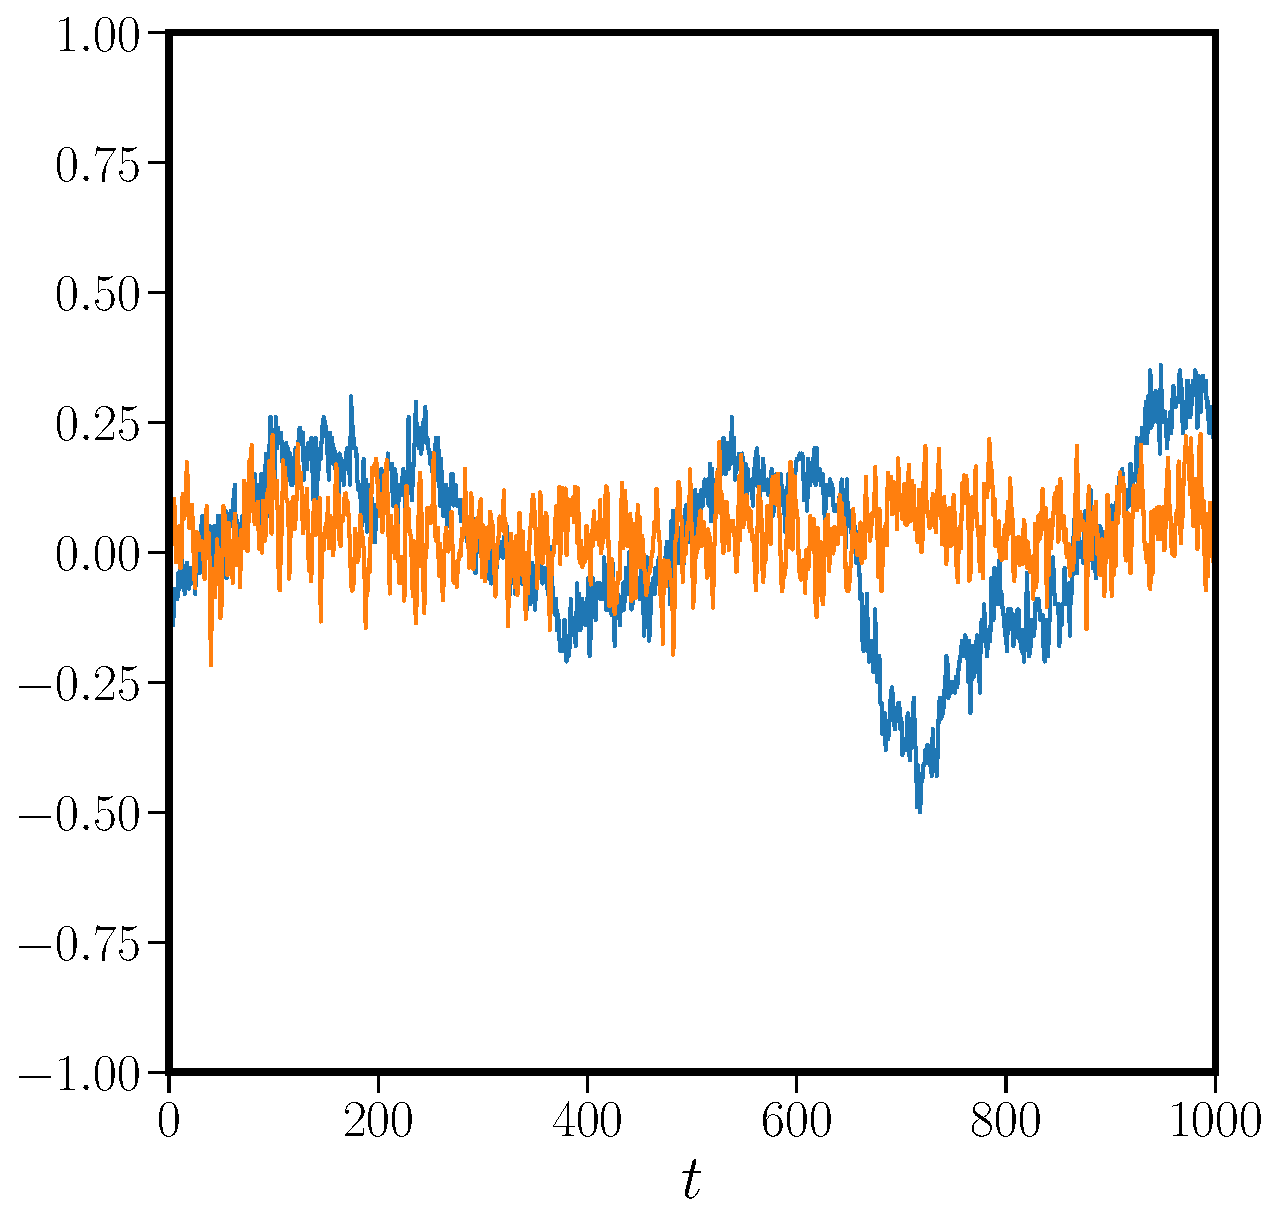
\includegraphics[width=\textwidth]{img/nabp/recap_mss/orderparameter_0.5_80_tau100.pdf}
        \end{minipage}
    \end{tabular}
    \caption[timedep_lolom]
    {
        オーダーパラメータの時間依存性。オレンジ色の線は$\psi(t)$を、青色の線は$V(t)$を表す。
        パラメータは$\varphi=0.5、R=10、M=80$とし、(a) $Pe=0.1$ 、(b) $Pe=10$、(c) $Pe=100$とした。
    }
    \label{fig:nabp_lodense_him_taudep_timedep}
\end{figure}




これらの結果をまとめるため、オーダーパラメータについて平均を取った結果が\figref{fig:nabp_lodense_psi_V}である。
この結果は、$\varphi=0.5、R=10$における、渦秩序変数$\psi$と規格化された角運動量$|V|$の
$Pe$および$M$依存性を表すグラフである。慣性が大きな$M=10,80$における結果について注目すると、
$\psi$、及び$|V|$の値は$Pe$によらず0.2を超えない小さな値を持つ。このことから、慣性が大きな領域ではその速度が乱雑な状態であることが分かる。
この状態は粒子の速度だけでなく、粒子配置についても無秩序な状態であり、これらの状態では円全体における大きな渦が生じないことが分かる。%TODO:M≒0.1について
\begin{figure}
    \centering
    \begin{tabular}{c}
        \begin{minipage}{0.4\hsize}
            \text{(a)}
            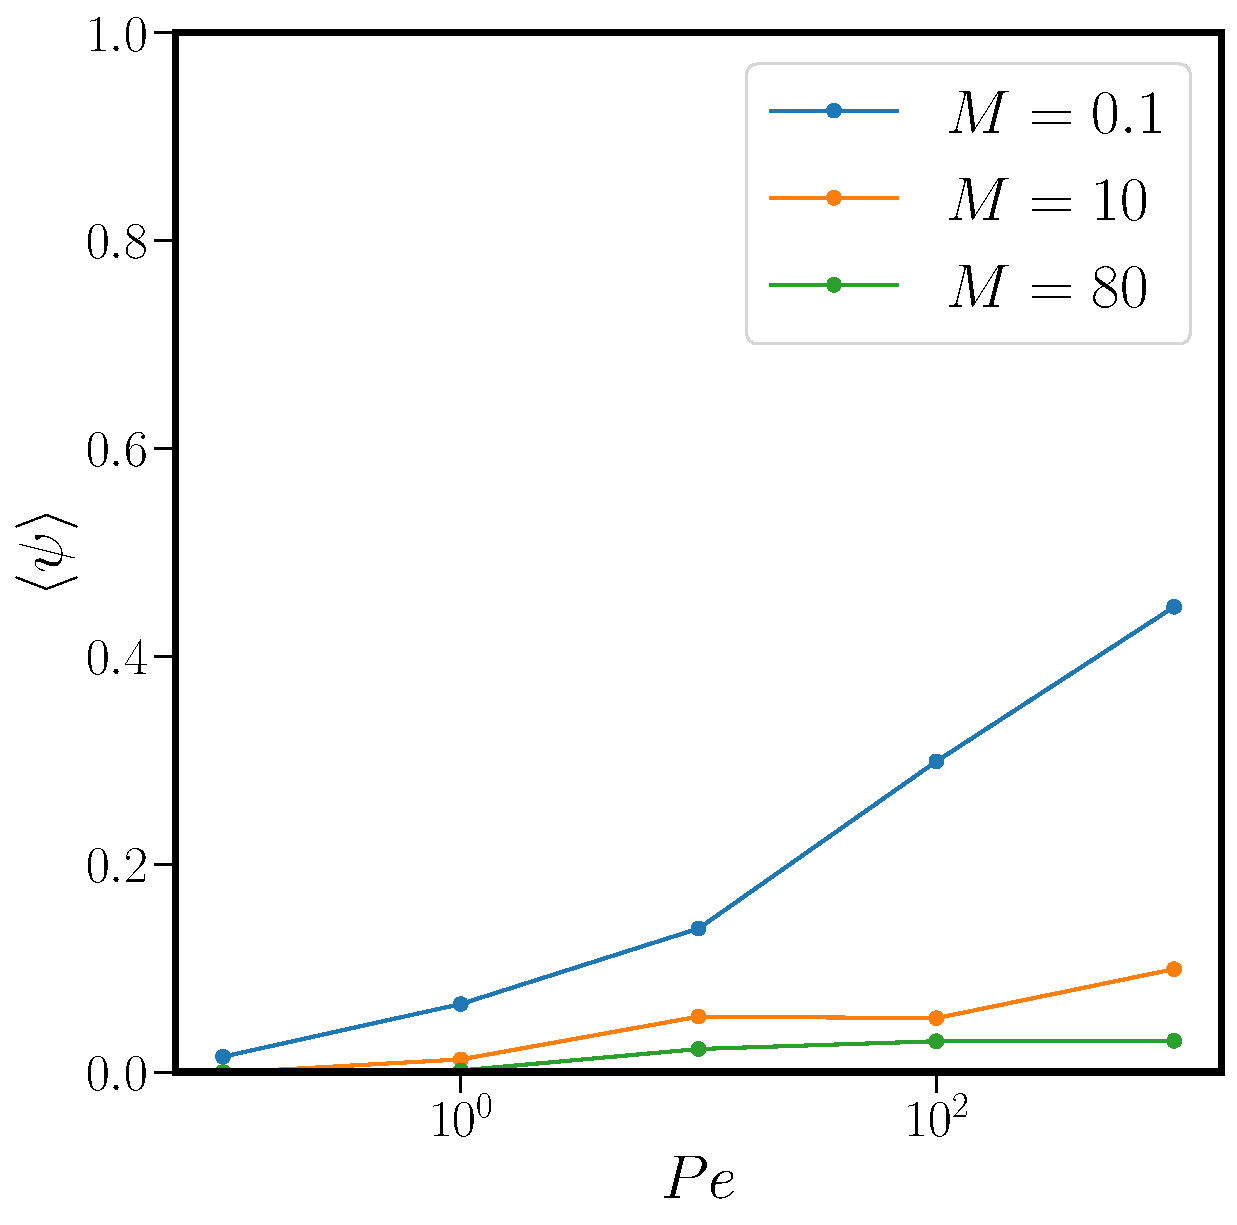
\includegraphics[width=\textwidth]{img/nabp/ens_r1/psi_0.5_[0.11080]_xsqFalse.pdf}
        \end{minipage}
        \begin{minipage}{0.4\hsize}
            \text{(b)}
            \includegraphics[width=\textwidth]{img/nabp/ens_r1/|V|_0.5_[0.11080]_xsqFalse.pdf}
        \end{minipage}
    \end{tabular}
    \caption[mdep_lodense]
    {
        $\varphi=0.5$におけるオーダーパラメータの$M$及び$Pe$依存性。
        (a) $\psi$ (b) $|V|$。系の半径$R=10$を選んだ。
    }
    \label{fig:nabp_lodense_psi_V}
\end{figure}

\subsubsection{高密度系}
低密度系では、慣性の小さい領域において MIPS が現れ、その影響を回避するため慣性を大きくすると粒子配置、及び速度は
無秩序になり、流れは見えなかった。
続いて、 MIPS による影響を回避するためのもう一つの方法として高密度の系について調べた。
具体的には密度を$\varphi=0.7$としてシミュレーションを行い、それらについて解析を行なった。

\figref{fig:nabp_highdense_him_taudep_timedep}は、慣性の大きな領域である$M=80$に関するオーダーパラメータ
$\psi、V$の時間依存性を表すグラフである。ここで、$R=10$と置いた。これらの図から、$Pe$の値を大きくしていくと$\psi$
の値が大きくなることが分かる。これは、$Pe$を大きくして系を非平衡に近づけるほど粒子は角度方向に向かって流れ、一つの渦へと近づいていくことを示す。
このことは$V$について注目することによっても確認することができる。$V$は$Pe$が大きくなるにつれてその絶対値が大きくなり、その符号を変えながら振動している。
このことは$Pe$の大きな$Pe=100$において、多くの粒子が同じ方向に向かって流れていることを意味する。また、符号が切り替わっていることから、
その流れの方向は時計回り、反時計回りの回転を繰り返していることが分かる。また、この流れが反転する時に注目すると
$\psi$も同時に0に近づいている。このことから、渦の向きが反転する時に一斉にその動きを変えるのではなく、ゆっくりと徐々にその向きを変えていることが分かる。

\begin{figure}
    \centering
    \begin{tabular}{c}
        \begin{minipage}{0.3\hsize}
            \text{(a)}
            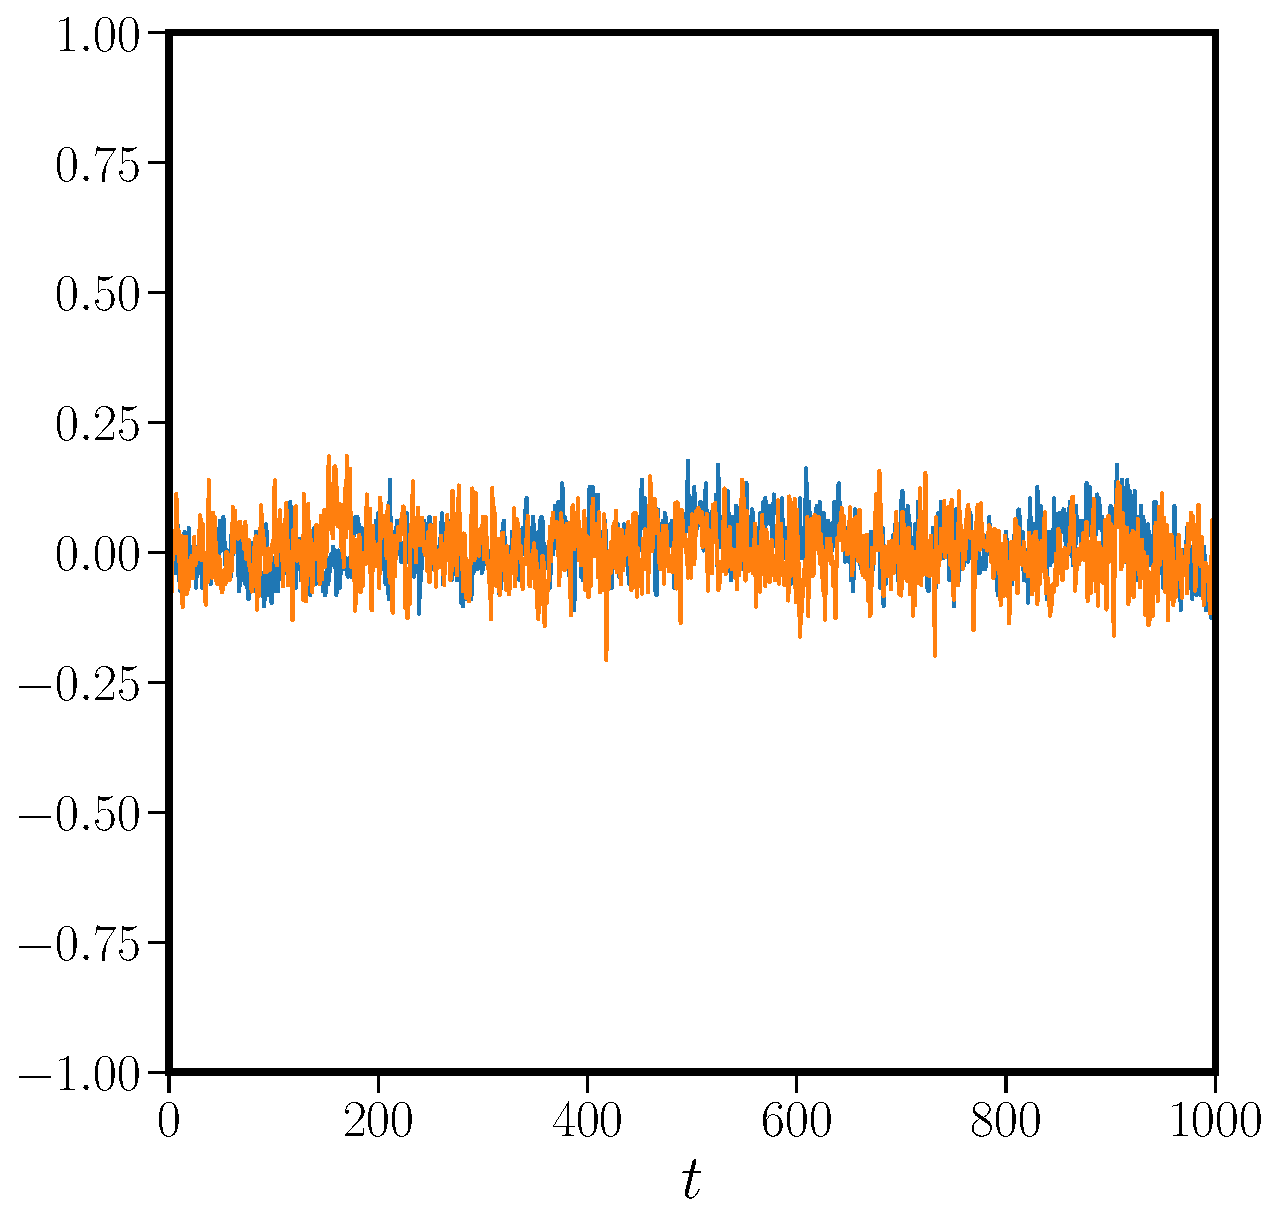
\includegraphics[width=\textwidth]{img/nabp/recap_mss/orderparameter_0.7_80_tau0.1.pdf}
        \end{minipage}
        \begin{minipage}{0.3\hsize}
            \text{(b)}
            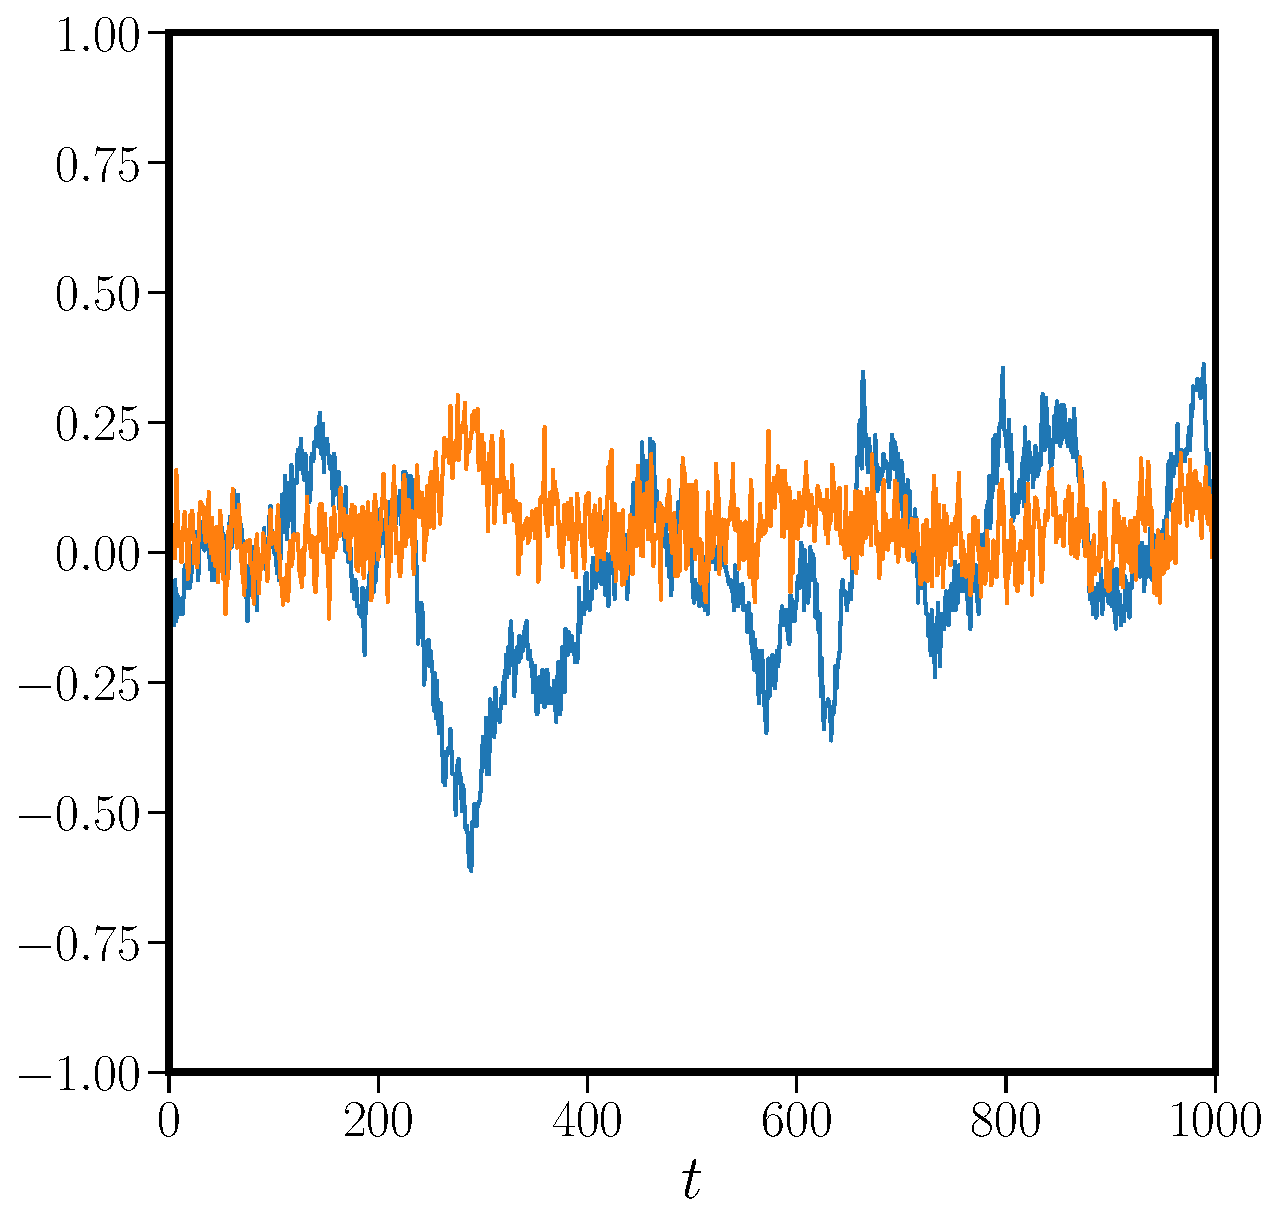
\includegraphics[width=\textwidth]{img/nabp/recap_mss/orderparameter_0.7_80_tau10.pdf}
        \end{minipage}
        \begin{minipage}{0.3\hsize}
            \text{(c)}
            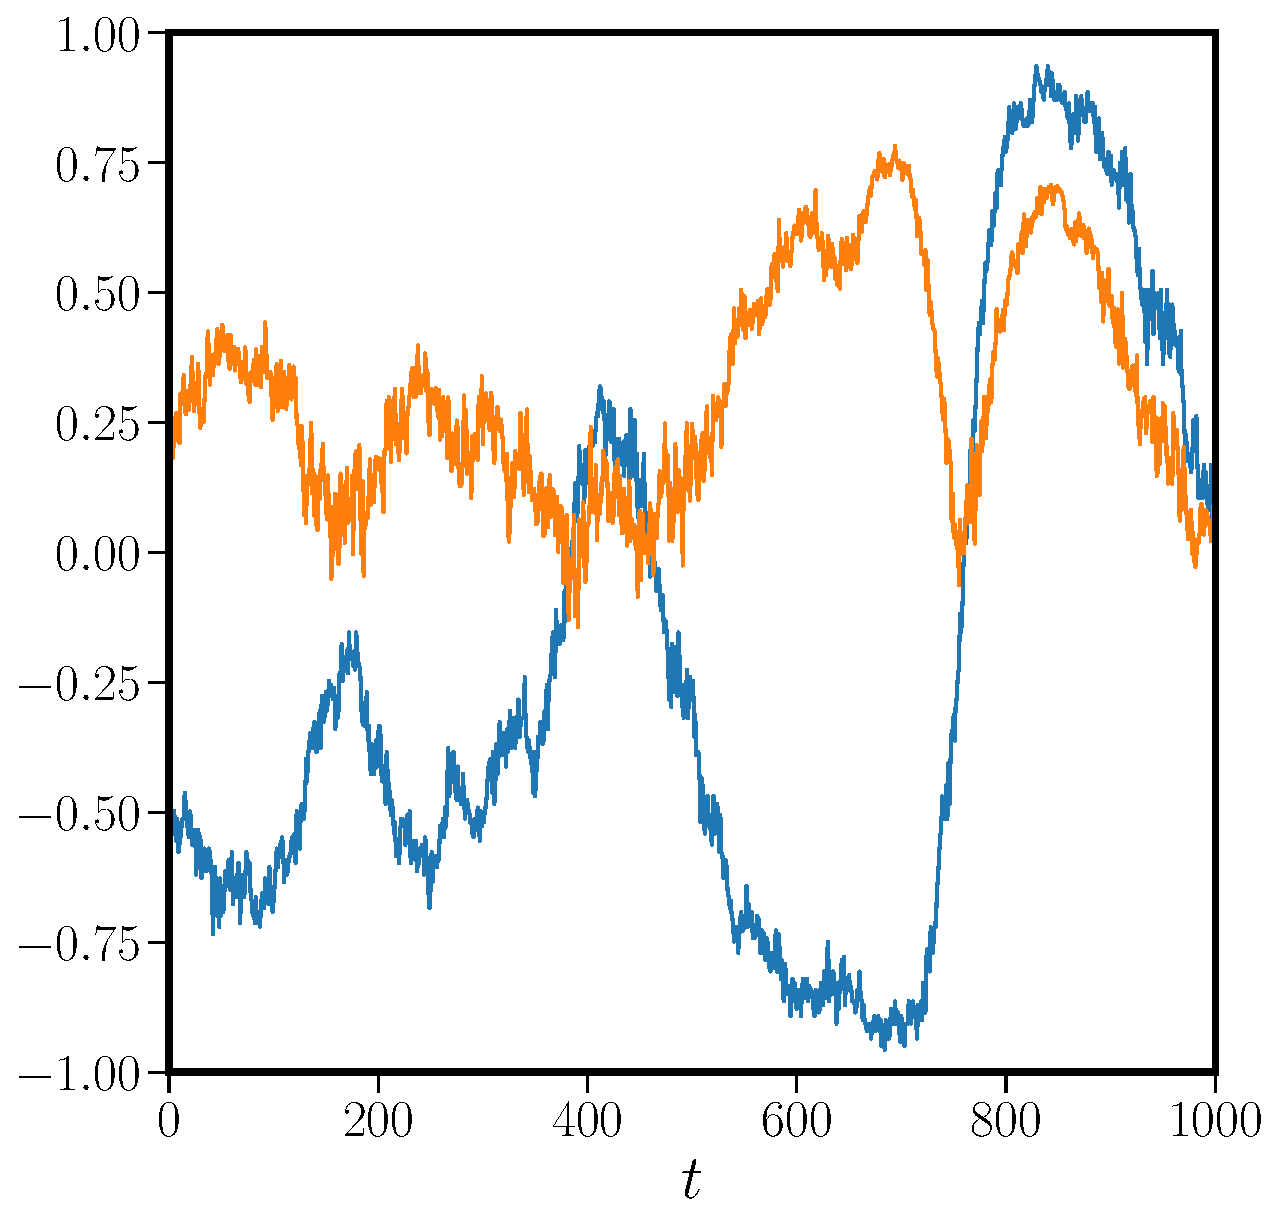
\includegraphics[width=\textwidth]{img/nabp/recap_mss/orderparameter_0.7_80_tau100.pdf}
        \end{minipage}
    \end{tabular}
    \caption[timedep_lolom]
    {
        オーダーパラメータの時間依存性。オレンジ色の線は$\psi(t)$を、青色の線は$V(t)$を表す。
        パラメータは$\varphi=0.7、R=10、M=80$とし、(a) $Pe=0.1$ 、(b) $Pe=10$、(c) $Pe=100$とした。
    }
    \label{fig:nabp_highdense_him_taudep_timedep}
\end{figure}


続いて、この系が低密度領域と同じように慣性の大きさによってその運動に定性的な違いがあるかどうかについて調べた。
慣性の小さな領域である$M=0.1$における結果を示す。\figref{fig:nabp_coor_highdense_mlo_taudep}はこの系における粒子配置、
\figref{fig:nabp_highdense_lom_taudep_timedep}はオーダーパラメータの時間依存性についてそれぞれ示す図である。
これらの図から、$Pe$の値を大きくしていくと$\psi$の値が大きくなることが分かる。
これは、$Pe$を大きくして系を非平衡に近づけるほど粒子は角度方向に向かって流れ、一つの渦へと近づいていくことを示す。
このことは$V$について注目することによっても同様に確認することができる。$V$の値は$Pe$が大きくなるに従ってその絶対値が大きくなり、
その符号を変えながら振動していることが分かる。これらの結果は、$Pe$を大きくするにつれて系全体が同じ方向に向かって流れ、
その流れの方向は時計回り、反時計回りに不規則に回転することを示す。


これらの結果は、慣性の効果が大きい$M=80$の系における結果と定性的に同じである。\figref{fig:nabp_highdense_him_taudep_timedep}と
\figref{fig:nabp_highdense_lom_taudep_timedep}を比べてみると、$Pe$を変化させた時のオーダーパラメータの値の変化は同じである。
慣性が大きい系においてはオーダーパラメータの時間変化は慣性が小さな系に比べて滑らかである。これは慣性が大きい場合、粒子への力が及ぼす座標の変化が
遅く伝わる効果によるものと考えられる。
これらの結果は、平均をとってその値を比較するとより理解することができる。
\figref{fig:nabp_vabs_lo0.7_m}は、$\varphi=0.7、R=10$における、渦秩序変数$\psi$と規格化された角運動量$|V|$について平均を取った値の
$Pe$および$M$依存性を表すグラフである。
まず$M$依存性について考えると、$\psi、|V|$のいずれのおいても
$M$が大きくなるにつれてパラメータの値が小さくなっていることが分かる。また各$M$における$Pe$依存性をみると、
$M$の変化によっては定性的には変化しなかった。この結果は、高密度系における iABP に対する慣性による効果を示している。
すなわち、その量は定性的な性質には影響を与えないということである。このことは、iABP における非平衡さは自己駆動項が支配しており、
慣性の影響は定量的には自己駆動力による働きを弱くする方向に働くものの、定性的にはその振る舞いに変化がないということを示している。
よって、以降は$M=0.1$のパラメータに注目して論じる。%考察?
次に$Pe$依存性に注目する。図から、$Pe$が大きくなると$\psi$及び$|V|$の値が大きくなる、
つまり粒子が同じ方向へと流れることがわかる。これは先行研究\cite{capriniCollectiveEffectsConfined2021}
におけるオーダーパラメータの変化と定性的に同じであり、同様のメカニズム、つまり系の持つ相関長が閉じ込めの半径よりも大きくなった場合に
粒子の運動の向きが揃う方向へと変化していると考えられる。しかし、本研究における$|V|$の絶対値は最大でも0.6であり、
先行研究\cite{capriniCollectiveEffectsConfined2021}より小さい値を取った。先行研究に比べると
発生した流れが安定していないことを示す。これは壁の形状によって生じる変化であると考えられる。先行研究では1次元のリング状の壁を用いており、
動径方向の運動が制限されており、粒子は角度方向に運動しない。しかし、本研究では2次元の円形領域を用いているため、粒子の運動は角度方向だけでなく
動径方向についても許されており、動径方向への運動が度々起こる。

このことは\figref{fig:nabp_vabs_lo0.7_m}(a)をみることでより理解できる。
この図から、$\psi$の値は最大でも0.5程度であることが分かる。この値は、系が完全に渦をなしている状態である1に比べると小さな値であり、
このことは粒子は角度方向だけでなく動径方向の運動も多くしており、その粒子配置を壊していることを示している。
\begin{figure}
    \centering
    \begin{tabular}{c}
        \begin{minipage}{0.3\hsize}
            \text{(a)}
            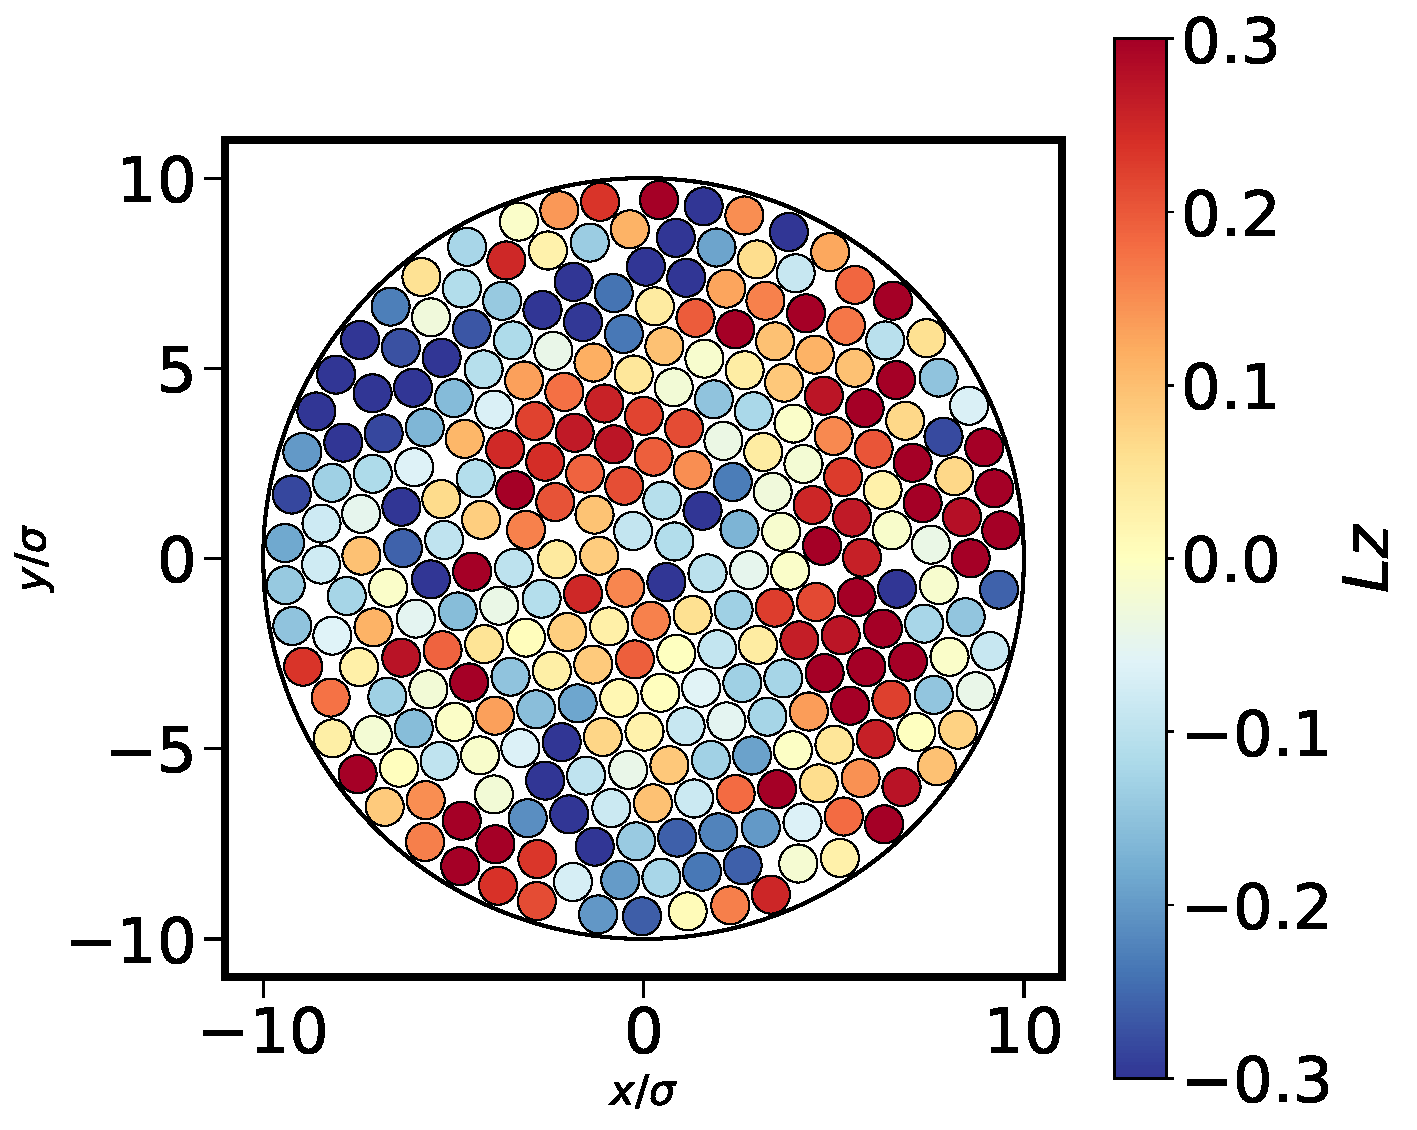
\includegraphics[width=\textwidth]{img/hloabp/ens_r1coor_R10_lo0.7_m0.1_tau0.1.pdf}
        \end{minipage}\begin{minipage}{0.3\hsize}
            \text{(b)}
            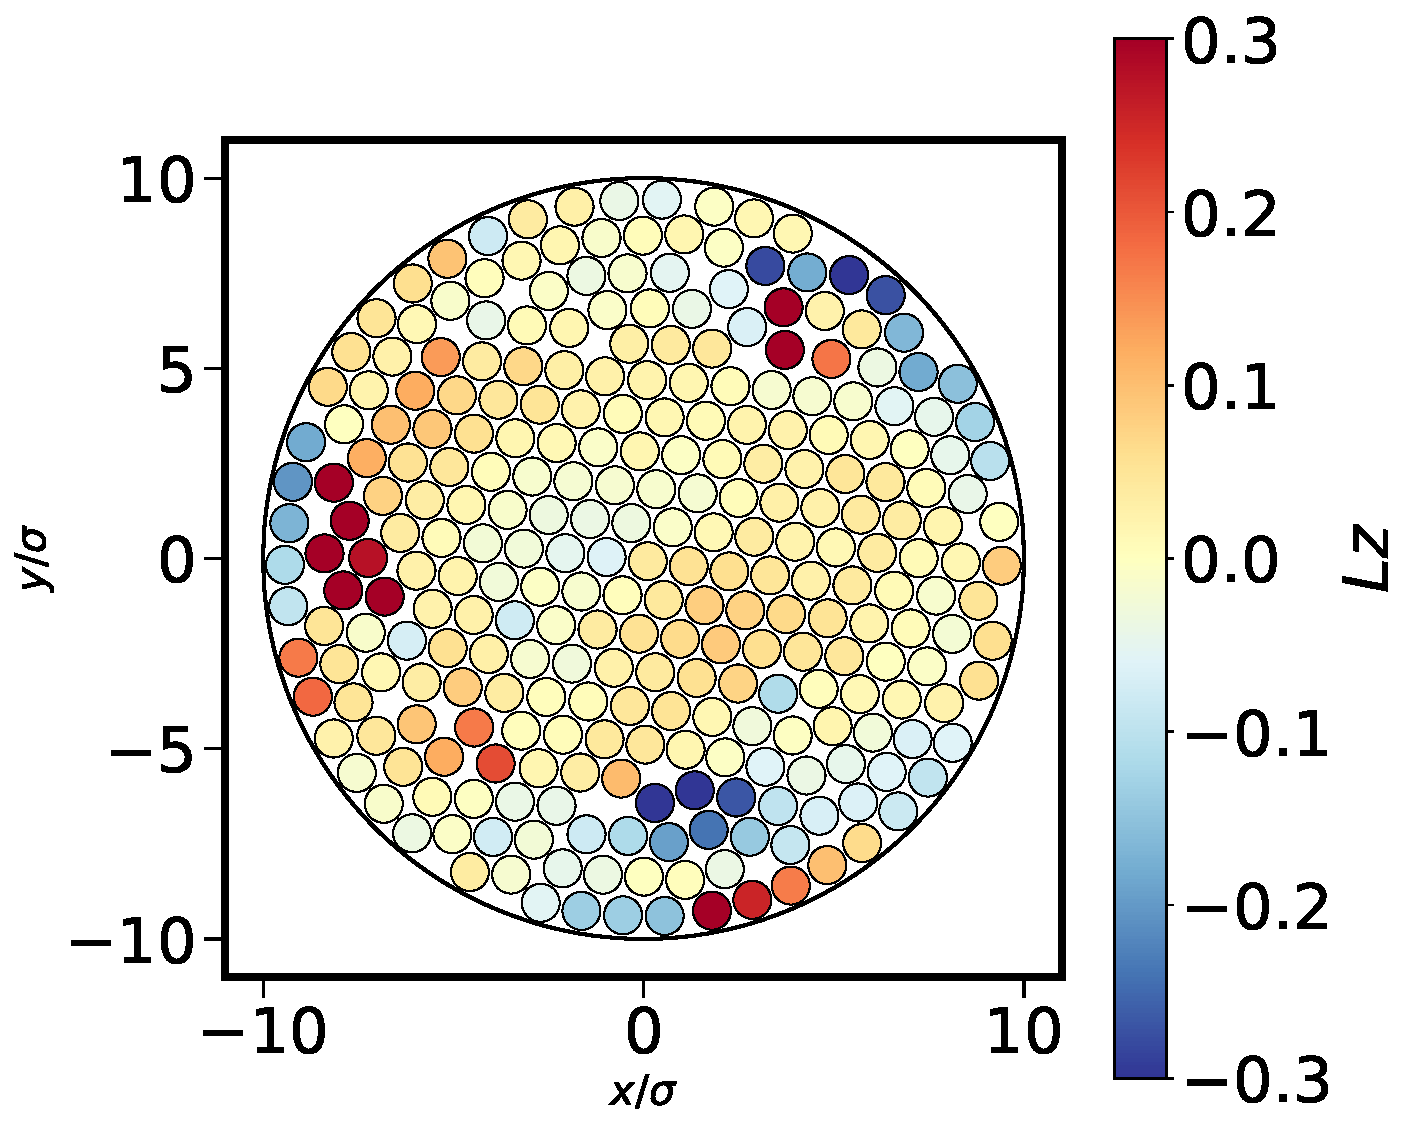
\includegraphics[width=\textwidth]{img/hloabp/ens_r1coor_R10_lo0.7_m0.1_tau10.pdf}
        \end{minipage}
        \begin{minipage}{0.3\hsize}
            \text{(c)}
            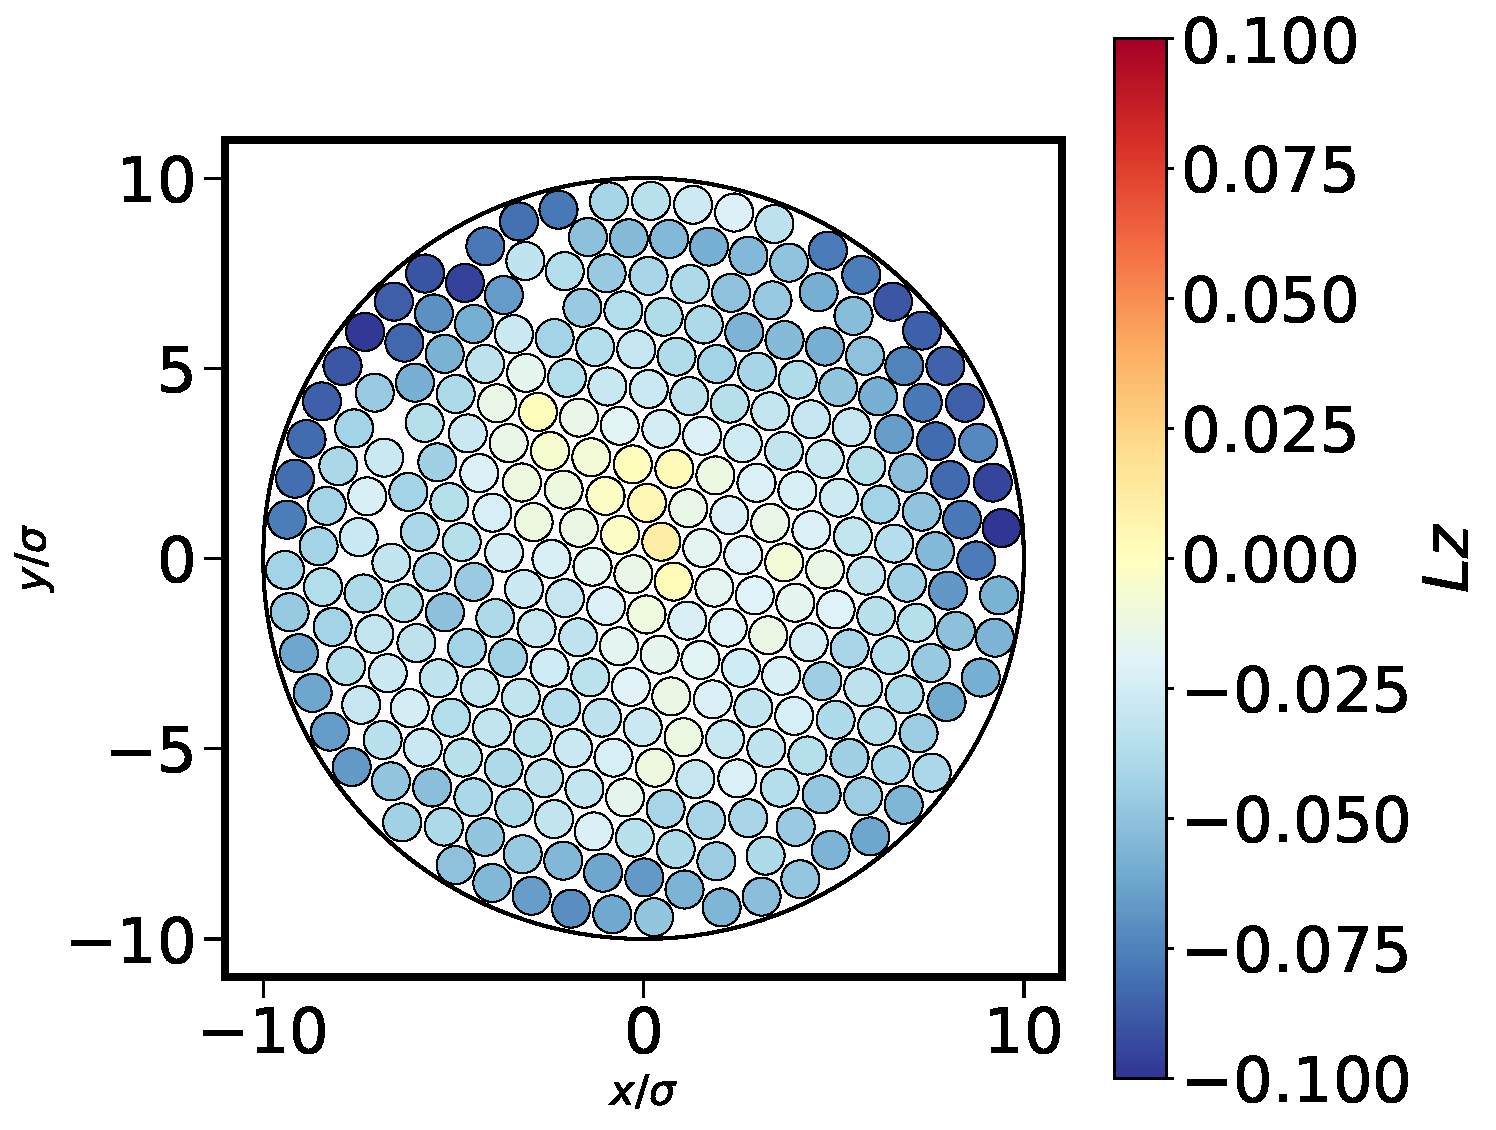
\includegraphics[width=\textwidth]{img/hloabp/ens_r1coor_R10_lo0.7_m0.1_tau100.pdf}
        \end{minipage}

    \end{tabular}
    \caption[coor_lo]
    {
        $\varphi=0.7、R=10$における粒子配置。各図において、粒子の色は各粒子の角運動量を表す。
        パラメータは$M=0.1$を用い、(a) $Pe=0.1$ (b) $Pe=10$ (c) $Pe=100$ である。
    }
    \label{fig:nabp_coor_highdense_mlo_taudep}
\end{figure}
\begin{figure}
    \centering
    \begin{tabular}{c}
        \begin{minipage}{0.3\hsize}
            \text{(a)}
            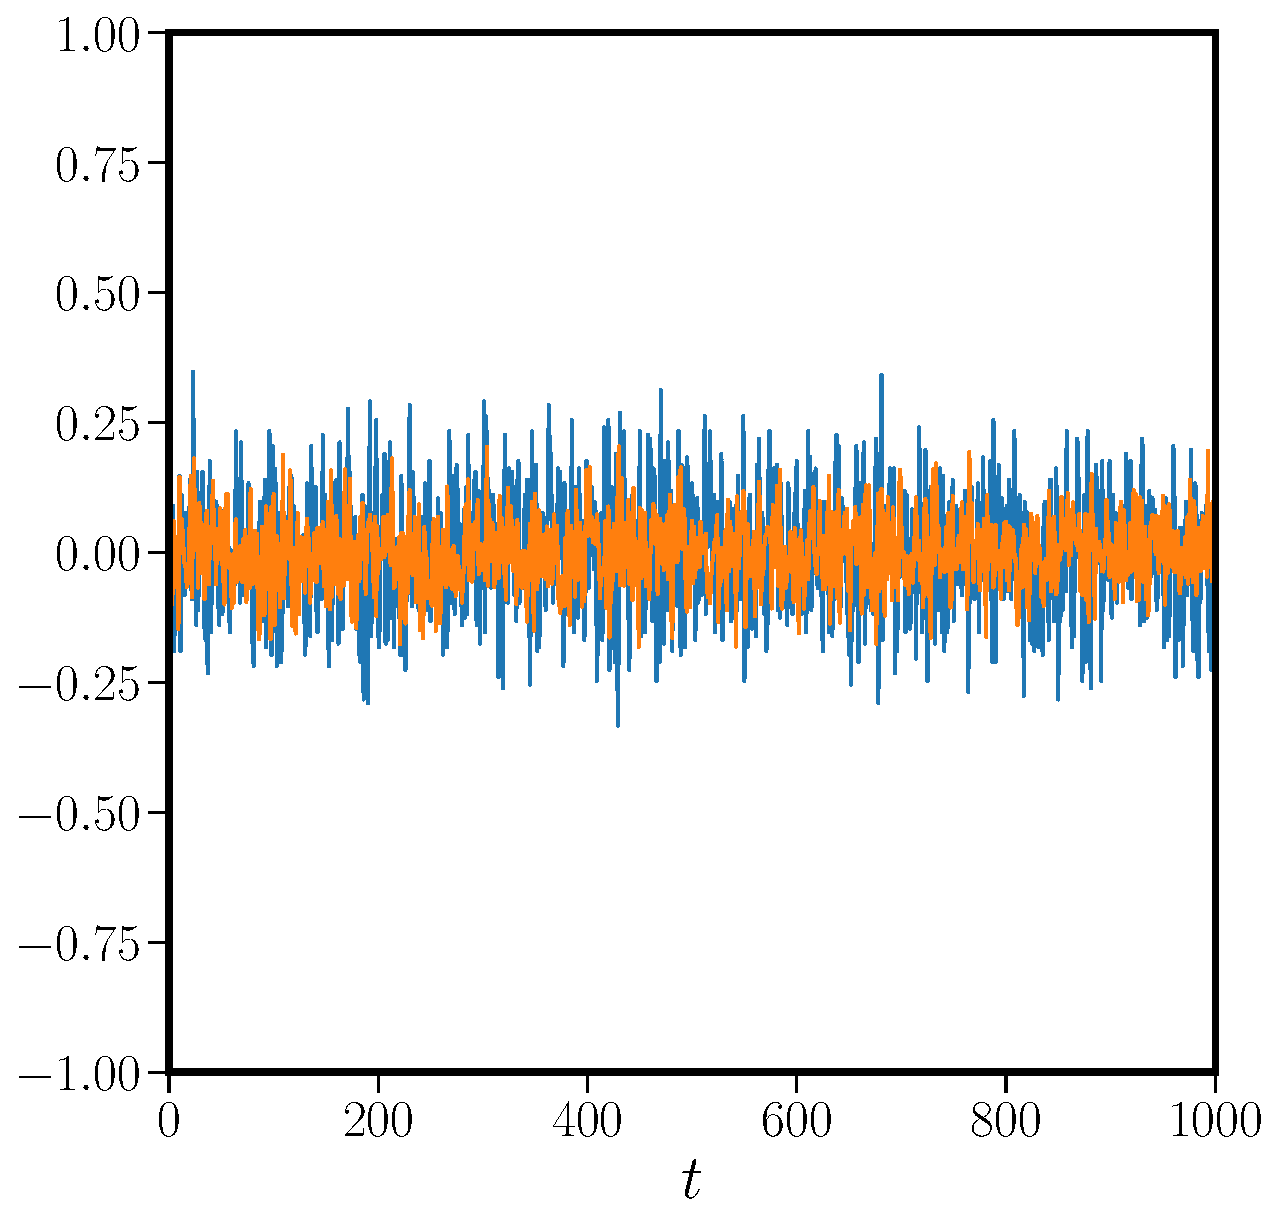
\includegraphics[width=\textwidth]{img/nabp/recap_mss/orderparameter_0.7_0.1_tau0.1.pdf}
        \end{minipage}
        \begin{minipage}{0.3\hsize}
            \text{(b)}
            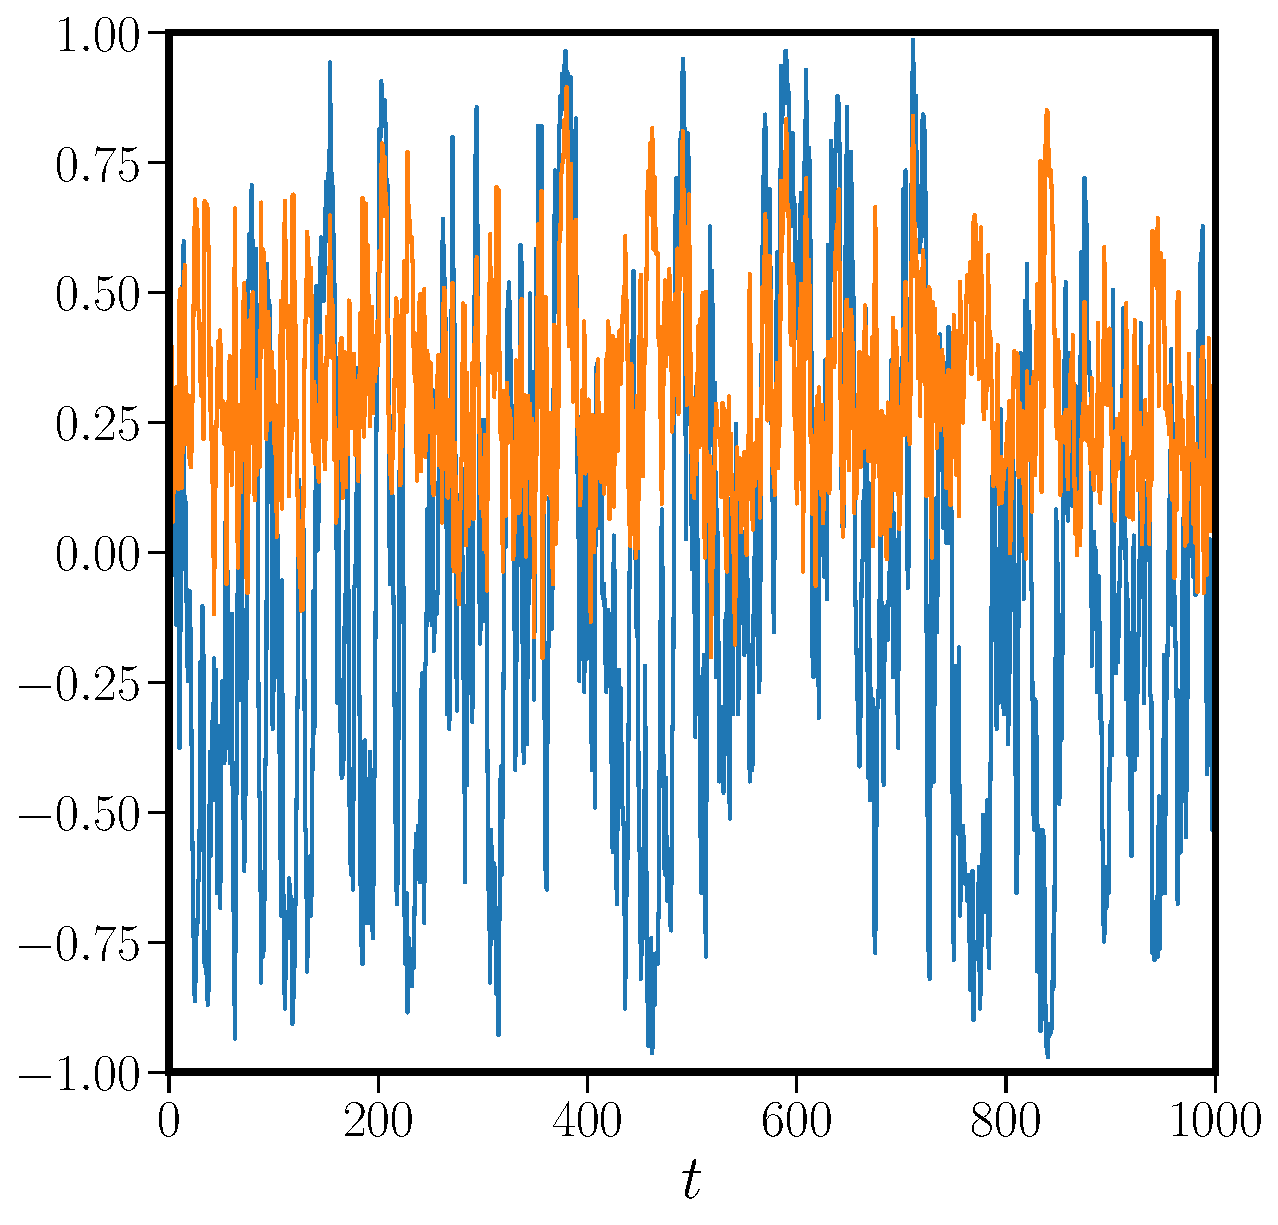
\includegraphics[width=\textwidth]{img/nabp/recap_mss/orderparameter_0.7_0.1_tau10.pdf}
        \end{minipage}
        \begin{minipage}{0.3\hsize}
            \text{(c)}
            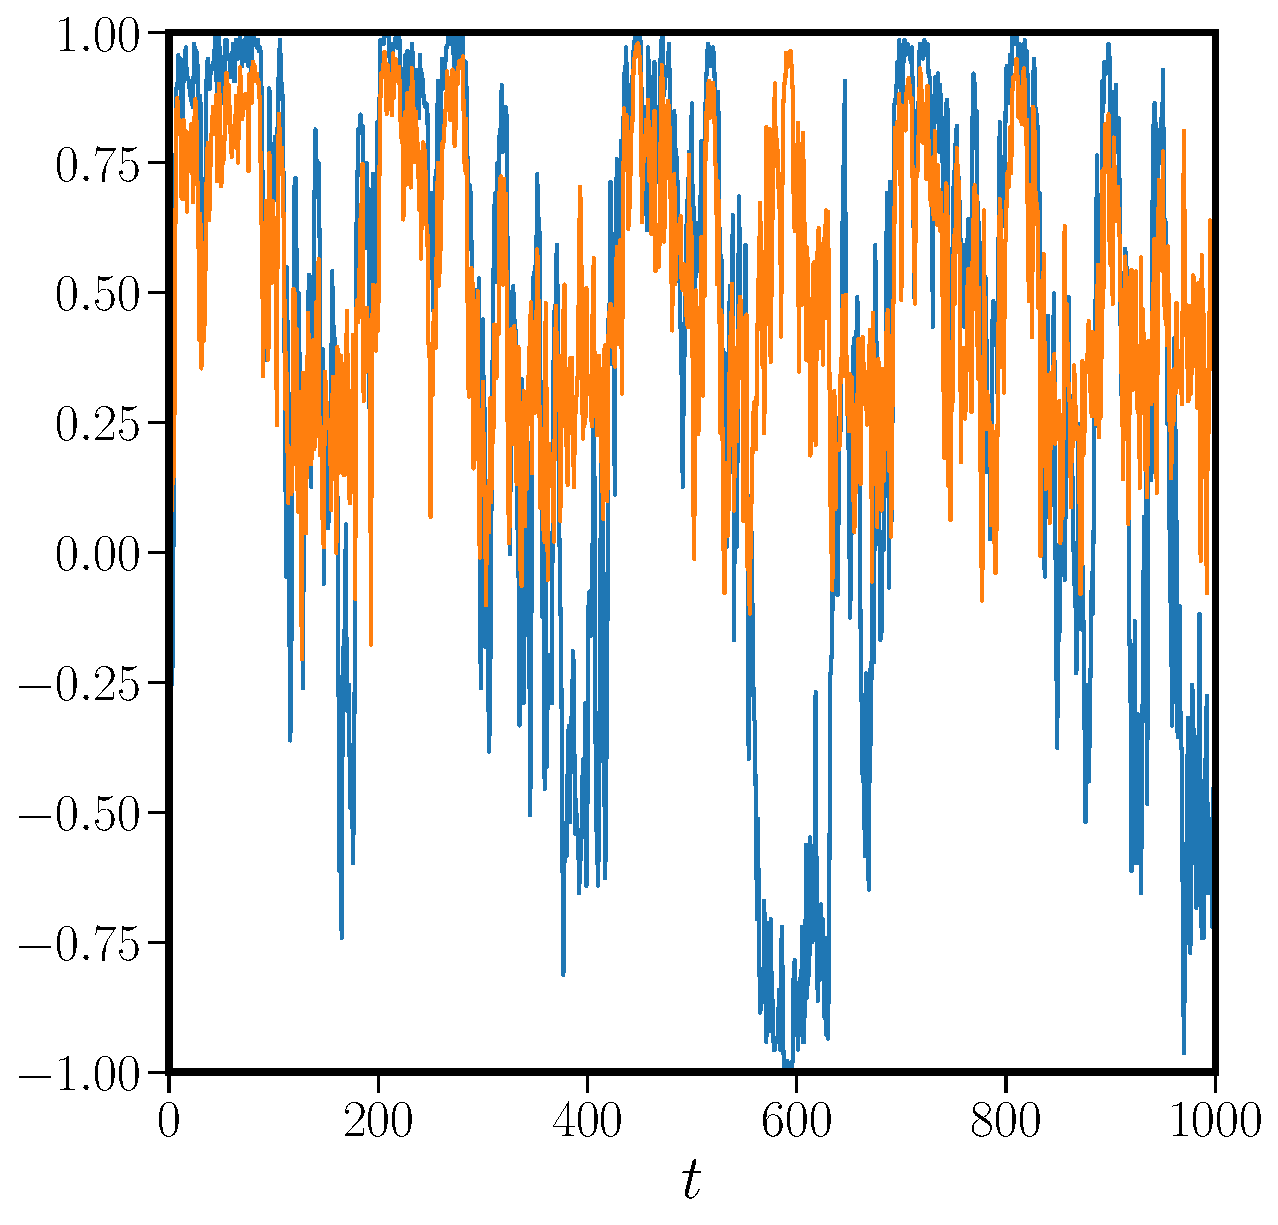
\includegraphics[width=\textwidth]{img/nabp/recap_mss/orderparameter_0.7_0.1_tau100.pdf}
        \end{minipage}
    \end{tabular}
    \caption[timedep_lolom]
    {
        オーダーパラメータの時間依存性。オレンジ色の線は$\psi(t)$を、青色の線は$V(t)$を表す。
        パラメータは$\varphi=0.7、R=10、M=0.1$とし、(a) $Pe=0.1$ 、(b) $Pe=10$、(c) $Pe=100$とした。
    }
    \label{fig:nabp_highdense_lom_taudep_timedep}
\end{figure}


\begin{figure}
    \centering
    \begin{tabular}{c}
        \begin{minipage}{0.4\hsize}
            \text{(a)}
            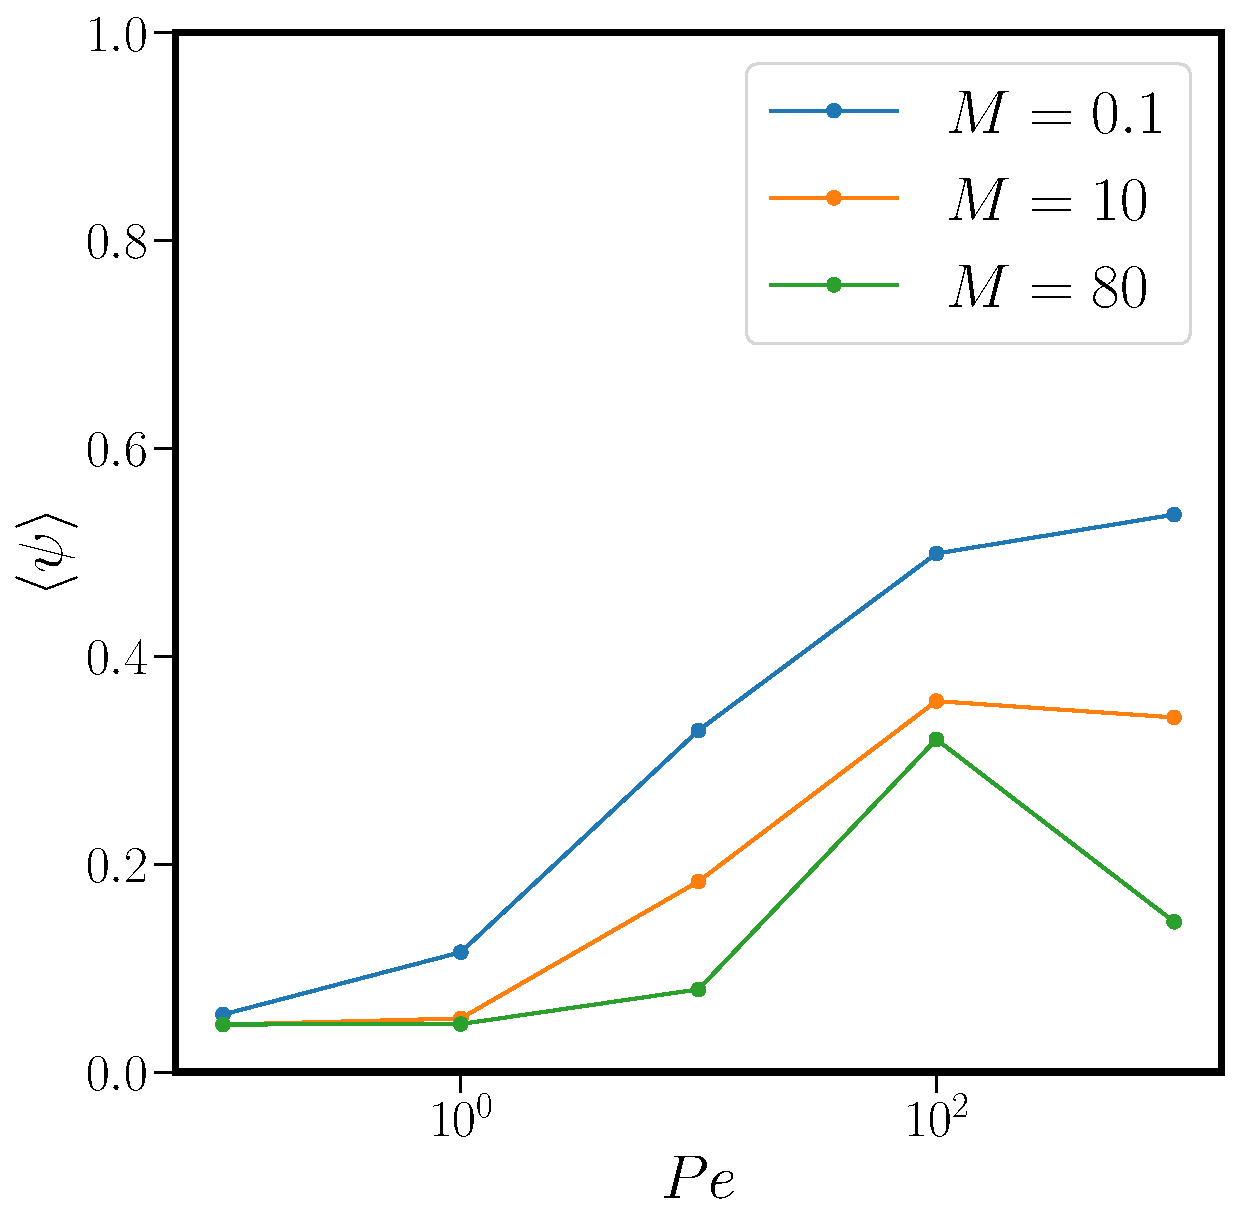
\includegraphics[width=\textwidth]{img/nabp/ens_r1/psi_0.7_[0.11080]_xsqFalse.pdf}
        \end{minipage}
        \begin{minipage}{0.4\hsize}
            \text{(b)}
            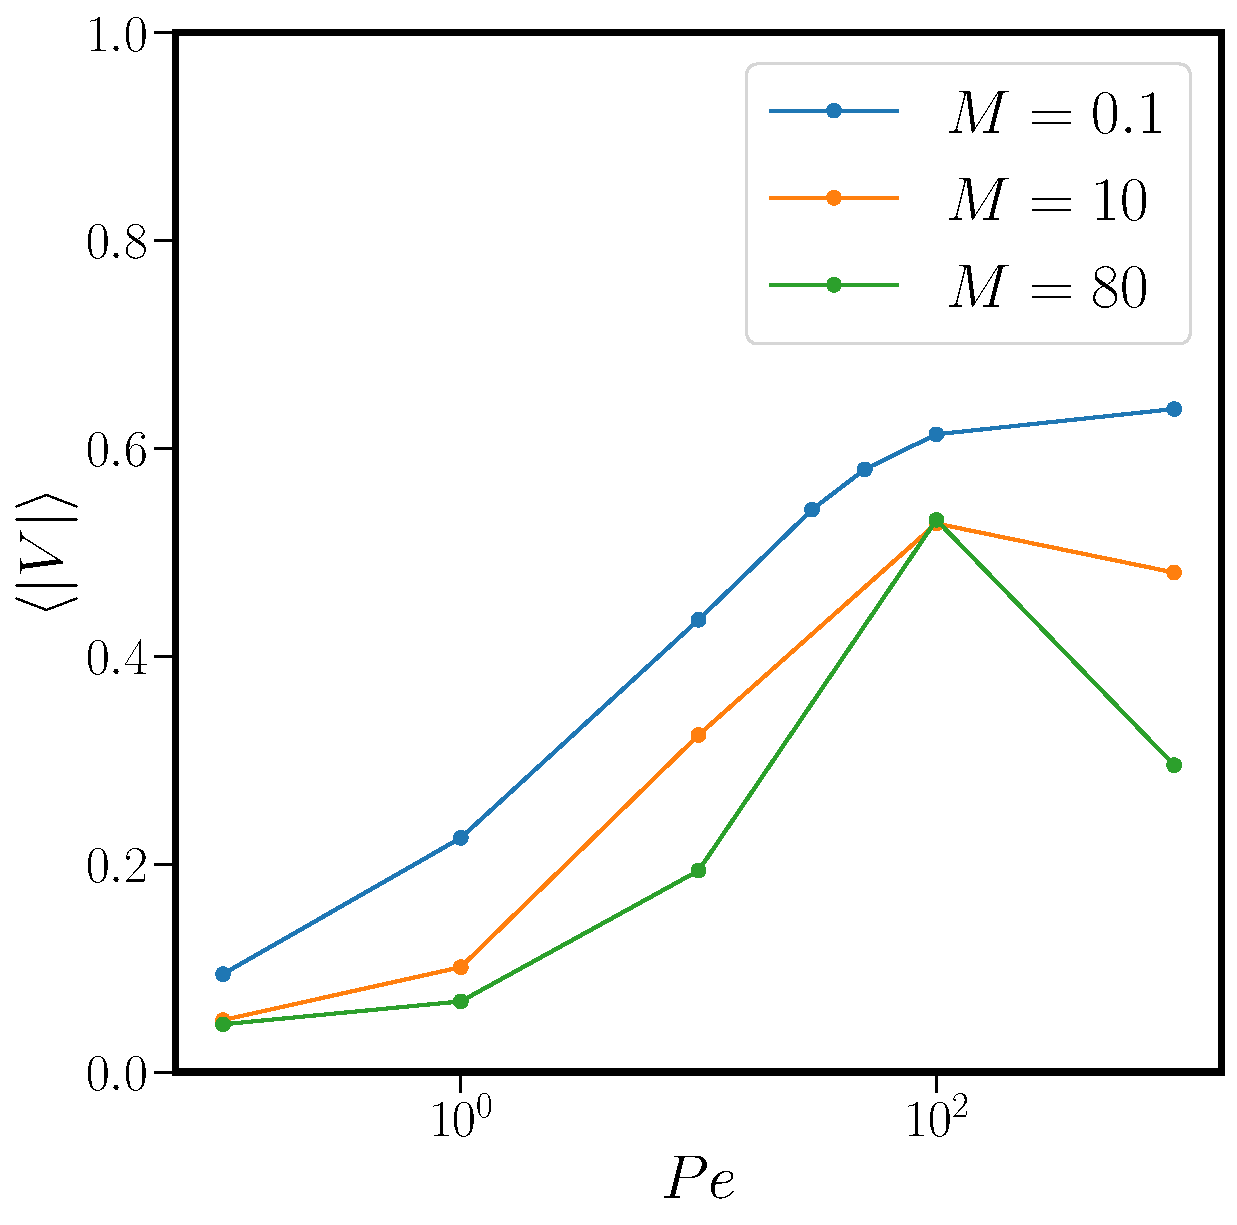
\includegraphics[width=\textwidth]{img/nabp/ens_r1/|V|_0.7_[0.11080]_xsqFalse.pdf.pdf}
        \end{minipage}
    \end{tabular}
    \caption[Four sample images]
    {
        $\varphi=0.7$におけるオーダーパラメータの$M$及び$Pe$依存性。
        (a) $\psi$ (b) $|V|$。系の半径$R=10$を選んだ。
    }
    \label{fig:nabp_vabs_lo0.7_m}
\end{figure}


\subsection{時間依存性}
\subsecref{subsec:result_nabp_holedinamics}では、高密度系において粒子はその運動方向を揃えて運動することがわかった。
その運動方向は定常的ではなく、時計回り、反時計回りの回転を繰り返していることが分かった。
この時間依存に関する\figref{fig:nabp_highdense_him_taudep_timedep}(c)をみると、$V$の値がその符号を正負に振動させており、その時間依存性は
周期的なものであり、一定の周期をもって振動しているように見える。


この時間依存性を定量的に評価するため、時間についてフーリエ変換を行った。
具体的には、系の全角運動量$L_z$に対してそのスペクトル$|L_z(\omega)|^2$、すなわち時間相関関数のフーリエ変換をとる。
この物理量は系の規則的な振動について計測するためのもので、系が一定の周期で振動しているとき、対応する周波数$\omega$に対してそのスペクトルに
ピークが現れる。

その結果が\figref{fig:fourie_transform}(a)である。
この図は密度$\varphi=0.7、M=0.1$における全角運動量のフーリエ変換のスペクトルを示した図である。
この図から、$Pe$が1より大きい領域では周波数$\omega$が大きな領域において、そのスペクトルが
$\omega^{-2}$に比例していることがわかる。これは一粒子状態のABPにおける速度相関のスペクトル\eqref{eq:intro_ft_about_iabp}
と一致する。実際に、$C(\omega)=C_0/(1+(\tau_{corr}\omega)^2)$でフィッティングした時の
$\tau_{corr}$と Péclet 数$Pe$の関係をプロットした図(\figref{fig:fourie_transform}(b))
を見ると分かる。%TODO::もう少し
この図から、$\tau_{corr}$が$ Pe$に比例することが分かる。これは一粒子状態のABPにおける速度相関のスペクトル%TODO:指揮をかく
と同様であり、これはこの系における系全体の回転の時間依存性は一粒子描像で描けることを示している。

\begin{figure}
    \centering
    \begin{tabular}{c}
        \begin{minipage}{0.4\hsize}
            \text{(a)}
            \includegraphics[width=\textwidth]{img/nabp/ens_r1/ft_lzlo0.7Ms0.1ta[0.1,1,30,50,100]Mg0R10Rbit0.0v021tmax1000.pdf}
        \end{minipage}
        \begin{minipage}{0.4\hsize}
            \text{(b)}
            \includegraphics[width=\textwidth]{img/nabp/ens_r1/ft_taucorr_lo0.7_m0.1.pdf}
        \end{minipage}
    \end{tabular}
    \caption[fourie_transform]
    {
        (a) $\varphi=0.7、M=0.1$ における$L_z$の時間についてのフーリエ変換。
        図中の点線は$\omega^{-2}$、及び$\omega^{-4}$に比例する直線を表す。
        (b) $C_0/(1+(\tau_{corr}\omega)^2)$でフィッティングした時の$\tau_{coor}$対$Pe$のグラフ
    }
    \label{fig:fourie_transform}
\end{figure}
また、\figref{fig:fourie_transform}(a)を見ると、$Pe=0.1$の時周波数$\omega$が大きな
領域で$\omega^{-4}$に比例している。これは$M=0.1$の系でシミュレーションを行なっており、
$M\simeq\tau_p$のため、慣性による緩和時間と自己駆動力による
緩和時間が等しいため起きていると考えられる。
\end{document}
